%% Target venue: The Journal of Computational Finance (Risk.net / Infopro Digital)
%% House style: author-date (Chicago) in-text; APA references with DOIs; abstract 150-200 words,
%% single paragraph, no citations; method-paper layout; <=10,000 words; double-blind (anonymized).
%% OPEN ITEMS: (1) anonymized title page on submission.
%% Table 4 (timing) + streaming row locked 2026-07-14 to one consistent quiet-machine
%% session (run512_*/run256_*, 5 reps each) under the FINAL build (-ffp-contract=off,
%% HH3 right chart, vectorized wing, rescue branch); every accuracy/bit-identity number
%% is final (regenerated 2026-07-13 on the same build). See BENCHMARK_PROTOCOL.md.
\documentclass[11pt]{article}
\usepackage[a4paper,margin=1in]{geometry}
\usepackage[T1]{fontenc}
\usepackage[utf8]{inputenc}
\usepackage{lmodern}
\usepackage{amsmath,amssymb,mathtools}
\usepackage{booktabs}
\usepackage{array}
\usepackage{microtype}
\usepackage{enumitem}
\usepackage{graphicx}
\usepackage{algorithm}
\usepackage{algpseudocode}
\usepackage{float}
\usepackage[authoryear,round]{natbib}
\usepackage[hidelinks]{hyperref}

\newcommand{\erf}{\operatorname{erf}}
\newcommand{\erfc}{\operatorname{erfc}}
\newcommand{\erfinv}{\operatorname{erf}^{-1}}
\newcommand{\erfcx}{\operatorname{erfcx}}
\newcommand{\PhiN}{\Phi}
\newcommand{\phiN}{\varphi}
\newcommand{\expmone}{\operatorname{expm1}}
\newcommand{\OTM}{\mathrm{OTM}}
% route tag: force medium-weight small caps so it renders even inside bold section titles
\newcommand{\rtag}[1]{{\normalfont\scshape #1}}

% Blind toggle: \blindtrue anonymizes for double-blind journal submission;
% \blindfalse produces the authored preprint (this is the repository/preprint build).
\newif\ifblind
\blindfalse

\title{A Routed, Vectorizable Table Inverter for\\ Machine-Precision Black--Scholes Implied Volatility}
\ifblind
  \author{}        % anonymized for double-blind review; separate title page
  \date{}
\else
  \author{Wolfgang Schadner\\[2pt]
    University of Liechtenstein\\[1pt]
    \texttt{wolfgang.schadner@uni.li}}
  \date{\today}
\fi

\begin{document}
\maketitle

\begin{abstract}
Recovering Black--Scholes implied volatility from an option price is among the most frequently executed numerical tasks in quantitative finance, increasingly demanded at machine precision and at vectorized-hardware throughput. We present a routed inverter that replaces data-dependent global iteration by regime-routed evaluation with fixed-count local refinements. The domain is decomposed into a central bivariate Chebyshev table in a transformed variable and three analytically matched endpoint charts whose special functions all reduce to a single two-parameter family. Each quote is routed by its IEEE-754 bit fields into branchless, fixed-operation-count kernels that the scalar and SIMD paths share identically, so batched evaluation reproduces the scalar result bit-for-bit across instruction sets and compilers. Against an independent 40-digit oracle, the worst relative error in volatility on the stated validation domain is $8.3\times10^{-16}$, matching the reference where both attain machine precision and holding that precision in the near-intrinsic and deep-wing regimes where the reference degrades. On a market-realistic S\&P~500 feed the vectorized inverter is $2.1$--$2.9$ times faster than the reference's public scalar implementation, and $3$--$9$ times faster on chart-pure fixed-moneyness batches, at bit-identical accuracy. Every representable input receives either a full-accuracy result or a flagged non-result.
\end{abstract}

\section{Introduction}
\label{sec:intro}

The implied volatility of a European option is the value of the volatility parameter that equates the Black--Scholes price to an observed market price. Because it is the coordinate in which option prices are quoted, compared, interpolated, and risk-managed, its computation is, in the words of \citet{jackel2006implication}, at once one of the most frequently executed and one of the least documented numerical tasks in derivatives modelling. A single recalibration of a volatility surface \citep{gatheral2006surface}, a local-volatility bootstrap, or a Monte Carlo pricing grid can require millions of inversions, and each must be accurate. An inverter that is correct only to a few digits injects noise into every downstream Greek and every calibrated parameter. The workload shape matters as much as the count. Production systems rarely invert one quote at a time. They invert a strip of strikes at one maturity, a whole surface, or a dense grid, and on modern hardware the difference between a method that processes such batches eight lanes at a time and one that cannot is a larger factor than any remaining difference in single-quote cost. That batch axis, not scalar latency, is where the present work aims.

Two largely separate literatures address the problem. The first seeks explicit, closed-form approximations to the inverse map. Early formulas supplied Newton seeds and near-the-money estimates \citep{manaster1982calculation,brenner1988simple,corrado1996note} and later work widened accuracy and domain. \citet{li2008approximate} fits rational functions of moneyness and maturity, \citet{stefanica2017explicit} derive an explicit formula with a uniform relative-error bound, and \citet{xiacui2018exact} an explicit series inversion. These are fast and naturally vectorizable, but they hold only on a bounded region of the input plane and only to modest precision. The second literature refines an initial guess to full machine precision. The reference method here is \citet{jackel2015rational}'s \emph{Let's Be Rational}, which combines a four-branch rational seed with two third-order Householder iterations on a carefully reformulated normalized Black function, and attains the last representable bit throughout the domain. Its accuracy is not in question. The cost is that a branch-rich, data-dependent iteration is difficult to vectorize, and its natural unit of work is a single scalar quote. A third, smaller strand precomputes the inverse map itself. \citet{glau2019chebyshev} interpolate the implied-volatility surface globally in Chebyshev polynomials, the approach closest in spirit to ours. \citet{matic2019pde} fit a polynomial table by a PDE method for batch-oriented use, but target an accuracy of $10^{-7}$, eight orders of magnitude short of the last bit.

The gap this leaves is a method that reaches machine precision \emph{and} vectorizes over the whole feasible domain, so that the batched workloads which dominate production (an entire book of quotes, or a dense calibration grid) run at hardware throughput rather than at scalar-iteration latency. We close that gap by treating inversion not as ``seed and refine'' but as \emph{routed evaluation with fixed-count local refinements}. Two regimes are pure table or series evaluations, the other two finish with a short \emph{fixed} number of correction steps, and no quote anywhere triggers a data-dependent iteration. The feasible region is partitioned into four regimes, each carrying an approximation in the coordinate natural to it. The interior is a central bivariate Chebyshev table in the transformed variable $W=h^2/2w$, whose cell geometry and polynomial degree follow a design principle fixed by the location of the inverse map's branch points and confirmed cell-by-cell by the fitted degrees. The three endpoint charts are a matched small-moneyness expansion built on the exact at-the-money kernel, an absolutely convergent large-volatility ladder, and an asymptotically peeled deep-wing inversion. A central structural result is that the special functions of all four charts are one two-parameter family, so the entire construction rests on a single evaluator plus the inverse error function. Every quote is routed into its regime by integer operations on its IEEE-754 bit fields, and evaluated by branchless kernels written so that the scalar entry point and the SIMD batch drivers execute the identical sequence of fused multiply-adds per quote. The batch result is therefore bit-for-bit identical to the scalar result, which we treat as a correctness invariant and verify exhaustively. Enforcing it requires a compiler discipline (Section~\ref{sec:simd}) that we believe is not widely appreciated. Under GCC's default floating-point contraction the same header can compile to two functions that differ in the last bit within one program.

Against an independent high-precision oracle the method attains a worst observed relative error in volatility of $8.3\times10^{-16}$ on the stated validation domain (Section~\ref{sec:setup}), matching Let's Be Rational wherever both are at machine precision and holding that precision in the two extreme regimes where the reference measurably degrades, and every representable input pair receives either a full-accuracy result or an explicitly flagged non-result. We also ask what a \emph{realistic} workload exercises. Routing an entire year of tradeable S\&P~500 index option quotes through the classifier shows the small-moneyness chart carrying about $90\%$ of that book and the deep wing a further $5\%$ (Section~\ref{sec:results}). That concentration is not a nuisance but a lever. A speculative driver exploits it (Section~\ref{sec:simd}) to invert a market-realistic S\&P~500 feed at $2.1$--$2.9$ times faster than the reference's official public scalar implementation, a qualification Section~\ref{sec:results} keeps explicit. A warm-restart driver serves the streaming regime at five to six times the reference, a deployment-mode figure under a documented few-ULP contract (Figure~\ref{fig:latency}). On tradeable quotes both solvers reach machine precision, so the case for the method on real data is throughput and determinism, with the accuracy advantage held in reserve for the extreme inputs a robust deployment must also handle.

\begin{figure}[htbp]
	\centering
	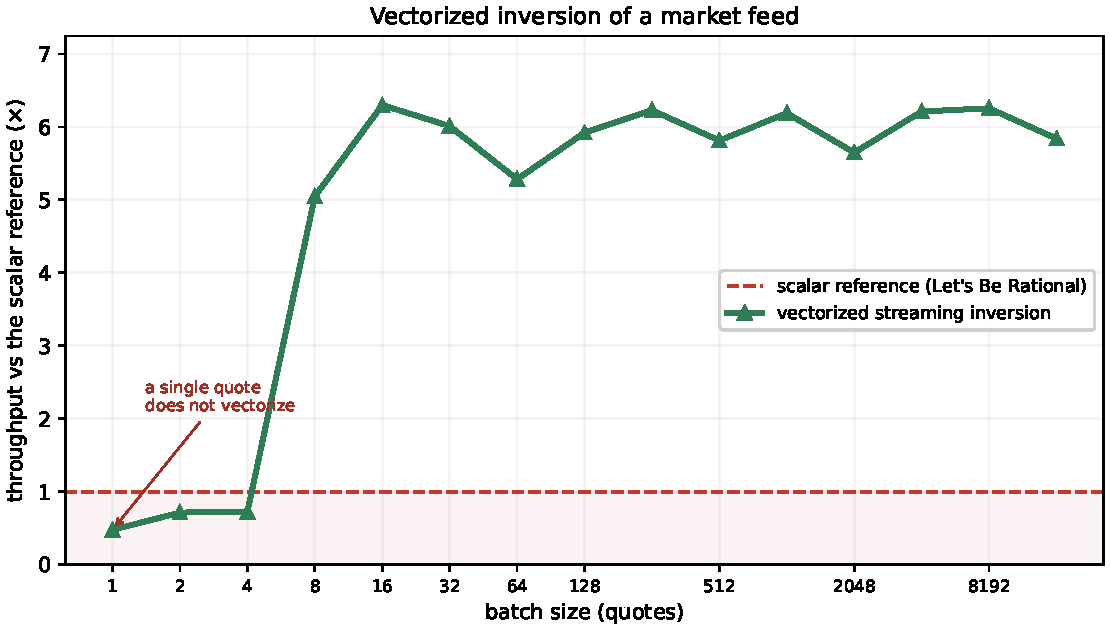
\includegraphics[width=0.78\textwidth]{fig_latency_batch}
\caption{Why vectorization is the point, on real data. Re-inverting a 2024 S\&P~500 book from the previous snapshot, the vectorized warm-restart driver of Section~\ref{sec:simd} sustains about five to six times the per-quote rate of the scalar reference solver, flat in batch size once a batch fills one SIMD register. This is a \emph{deployment-mode} comparison, the warm driver starts from each node's previous root, under its few-ULP contract (Section~\ref{sec:simd}). The like-for-like cold full-accuracy figure is $2.1$--$2.9$ times on the same feed (Table~\ref{tab:timing}). A single isolated quote cannot be vectorized and is the one regime the scalar reference still wins. Throughput is measured against the reference in the same session, so the host clock cancels.}
	\label{fig:latency}
\end{figure}

The paper is organized as follows. Section~\ref{sec:overview} states the method in brief. Section~\ref{sec:setup} fixes the normalized problem. Section~\ref{sec:approx} constructs the central table and the branch-point argument that sizes it, then the endpoint charts, their unification, and the accurate-forward evaluation. Section~\ref{sec:simd} describes routing and the scalar/SIMD bit-identical implementation. Section~\ref{sec:results} reports accuracy and performance, and Section~\ref{sec:conclusion} concludes.

\section{The method at a glance}
\label{sec:overview}

The method has two phases. An offline phase, run once, fits and freezes every coefficient of the central table and the endpoint charts. A runtime phase then routes each quote into its regime by integer tests on its IEEE-754 bit fields and evaluates it with a fixed, branch-free operation count. Algorithm~\ref{alg:overview} states both phases as a high-level summary. The construction is developed in Sections~\ref{sec:approx} and~\ref{sec:simd} and detailed in Appendices~\ref{app:hotpath} and~\ref{app:generation}.

\begin{algorithm}[H]
	\caption{The routed inverter at a glance}
	\label{alg:overview}
	\begin{algorithmic}[1]
\Statex \textbf{Offline (run once, detailed in Appendix~\ref{app:generation}).} From the branch-point principle of Section~\ref{sec:table}, fix the cell geometry. Fit the central Chebyshev table, the $B^{-1}$, $V_2$, $V_4$, wing and seam polynomials against 40-digit oracles. Gate every cell at $10^{-15}$ relative in $\sigma$. Freeze all coefficients as hexadecimal doubles.
\Statex \textbf{Runtime (per batch of quotes $(h_i, c_i)$).}
\State classify each quote by IEEE-754 bit fields and three frozen seam polynomials into \textsc{Central} / \textsc{Left} / \textsc{Right} / \textsc{Wing} (Section~\ref{sec:unify}). No price is evaluated to route
\State bucket quotes by chart (counting sort), or, when a sampled probe shows the small-moneyness share is high, evaluate \textsc{Left} speculatively on all lanes and defer only the minority
\For{each bucket, eight (AVX-512) or four (AVX2) quotes per SIMD register}
\State \textsc{Central}: bivariate Clenshaw sweep in $(x_h, x_\lambda)$, $w = h^2/(2W)$
\State \textsc{Left}: $A=B^{-1}(c/\expmone(h))$, matched expansion in $s=h/A$
\State \textsc{Right}: rational seed $+$ ladder $+$ exactly three Householder steps
\State \textsc{Wing}: peeled log-price equation, exactly six Newton steps
\EndFor
\State scatter results to input order. Every kernel is a branchless fused-multiply-add chain shared with the scalar entry, so the batch output is bit-identical to scalar
	\end{algorithmic}
\end{algorithm}

\section{The normalized inversion problem}
\label{sec:setup}

We work throughout with the normalized out-of-the-money (OTM) Black price \citep{blackscholes1973,merton1973rational}. Writing $h=|\log(K/F)|\ge0$ for the absolute log-moneyness, $w=\sigma^2T$ for the total variance and $v=\sqrt{w}=\sigma\sqrt{T}$ for the total standard deviation, the normalized OTM price is
\begin{equation}
  c \;=\; \PhiN\!\Big(\tfrac{v}{2}-\tfrac{h}{v}\Big)
        - e^{h}\,\PhiN\!\Big(-\tfrac{v}{2}-\tfrac{h}{v}\Big)
  \;\in\;(0,1),
  \label{eq:otm}
\end{equation}
with $\PhiN$ the standard normal cumulative distribution function. Calls and puts map to the same problem by the put--call symmetry $h\mapsto-h$, so it suffices to treat $h\ge0$, and the inversion problem is to recover $w$ (equivalently $\sigma$) from a given pair $(h,c)$. The reduction from raw option data deserves an exact statement, since \eqref{eq:otm} is written for the out-of-the-money \emph{call} ($K\ge F$). An in-the-money option first maps to its out-of-the-money twin by put--call parity, an out-of-the-money \emph{put} ($K<F$) is the dual call with $F$ and $K$ exchanged, and the surviving premium is normalized by $\min(F,K)$. The resulting $(h,c)$ satisfies \eqref{eq:otm}. The wrapper of Section~\ref{sec:simd} implements exactly this map. It is the same reduction used by \citet{jackel2015rational}, save that the normalizer is $\min(F,K)$ rather than $\sqrt{FK}$, a choice that matters in the deep wing (Section~\ref{sec:results}).

All of the analysis below flows from a single integral representation of \eqref{eq:otm}. Differentiating the Black price with respect to the total standard deviation and integrating back gives the exact form
\begin{equation}
  c \;=\; C(h,v) \;=\; k\,e^{h/2}\int_0^{v} e^{-t^2/8}\,e^{-h^2/(2t^2)}\,\mathrm{d}t,
  \qquad k=\frac{1}{\sqrt{2\pi}},\qquad C(h,\infty)=1,
  \label{eq:baseint}
\end{equation}
in which the integrand is the product of a Gaussian factor $e^{-t^2/8}$, regular at $t=\infty$, and a boundary-layer factor $e^{-h^2/(2t^2)}$ that vanishes to all orders at $t=0$. The two factors are the two endpoints of the inversion problem. The layer at $t=0$ governs the small-price wing, and the regular tail governs the large-volatility limit $c\to1$. The interior, where neither factor simplifies, is where a table is the natural device. Section~\ref{sec:table} treats the interior and Sections~\ref{sec:left}--\ref{sec:wing} the two endpoints.

The map \eqref{eq:otm} is analytic and strictly monotone in $v$, but it is numerically treacherous at both ends of the price range. As $v\to0$ the OTM price collapses like $c\sim \varphi(h/v)\,v/h$, so a plain Newton iteration on $c-C(h,v)$ has a vanishing derivative and loses all its significant digits. As $v\to\infty$, $c\to1$ and the two terms of \eqref{eq:otm} cancel. Robust inversion therefore requires working in a variable in which the map is well conditioned. The organizing object is the endpoint factorization of \eqref{eq:otm}: with the exponential scale variable
\begin{equation}\label{eq:Wdef}
  W \;=\; \frac{h^2}{2w} \;=\; \frac{h^2}{2v^2},
\end{equation}
one has the exact representation $c=\gamma(h)\,e^{-W}W^{-3/2}H(W)$, in which $\gamma(h)=\tfrac{h}{2}e^{h/2}/(2\sqrt\pi)$, and $H$ is an elementary, error-function-free convergent integral with $H(W)\sim1-(a+\beta)/W+\dots$ for a fixed pair $(a,\beta)=(3/2,h^2/16)$. This factorization is the deep-wing form of the generalized-inverse-Gaussian quantile representation of the Black map established in \citet{schadner2026explicit}, where the normalized OTM price is identified as a generalized-inverse-Gaussian distribution in the variance. Viewed as a function of a complex price, the inverse map continues analytically onto a ring-shaped domain (an \emph{annulus}) in the $c$-plane bounded by two circles, one passing through each of the branch points $c=0$ and $c=1$. The variable $W$ is the one in which the small-price behaviour is smooth, and it is the variable the central table stores.\\

It is worth recording at the outset what accuracy is even attainable. Writing $\nu(h,v)=\partial C/\partial v$ for the normalized vega, a relative perturbation $\varepsilon$ of the input price moves the exact root by the relative amount $\kappa\,\varepsilon$ with $\kappa=c/(v\,\nu)$, the relative condition number of the inversion. From \eqref{eq:baseint}, deep in the wing $\log c\approx-W$ so $\kappa\approx1/(2W)$, which is \emph{small}. The wing is benignly conditioned in relative terms, and there is no obstruction to recovering $\sigma$ to machine precision from prices as small as the smallest positive doubles. Near the upper endpoint the price itself is the wrong variable, since $\kappa\to\infty$ as $c\to1$, but the \emph{complement} $1-c$ is again benignly conditioned, with a relative perturbation of $1-c$ moving the root by only $\mathcal{O}(v^{-2})$ times as much. The design consequence, which recurs throughout the paper, is that full accuracy is attainable everywhere provided every formula works with whichever of $c$ and $1-c$ is small. Since the public entry takes only $c$, one point deserves precision. For $c\ge\tfrac12$ the subtraction $1-c$ is \emph{exact} by Sterbenz's lemma \citep{muller2018handbook}, so forming the complement loses nothing beyond the loss already committed when the caller rounded the price. The design rule is that no subsequent formula amplifies that rounded complement through an ill-conditioned intermediate. The reference solver of \citet{jackel2015rational} makes the same conditioning observation for its own normalization. The residual differences reported in Section~\ref{sec:results} arise where the two implementations' internal variables condition differently. One bound, however, no algorithm can cross. A caller who passes the price as a plain double has already rounded $1-c$, and once $v\gtrsim8$ that rounding alone moves the root by more than $10^{-13}$, growing to $10^{-3}$ near $v\approx16.6$ where $1-c$ reaches machine epsilon. This is a property of the input representation, shared by every double-precision inverter including the reference. The implementation surfaces it explicitly through a status flag rather than refusing the input (Section~\ref{sec:simd}).

We score accuracy as the relative error in $\sigma$ against an independent arbitrary-precision oracle, never against a round trip through a forward pricer. The forward map \eqref{eq:otm} loses precision to cancellation near $c\to0$ and $c\to1$, so re-pricing a computed $\sigma$ and comparing conflates forward-pricer error with inverter error and can inflate the apparent error of \emph{any} correct inverter by two orders of magnitude in the wings. The oracle instead inverts the \emph{given} double-precision price $c$ at 40 significant digits.

Throughout the paper, \emph{machine precision} means a relative error in $\sigma$ below $10^{-15}$ (at most a few units in the last place of a double) as \emph{observed on the stated validation sets}. The worst case recorded anywhere in Section~\ref{sec:results} is $8.3\times10^{-16}$, about five ULP. The claim applies on an explicit domain $\mathcal{D}$: feasible $(h,c)$ with $v=\sigma\sqrt T\le8$ and $h\le16.2$, extended by the rescue band of Section~\ref{sec:wing} ($h\le16.5$, $W\lesssim40$). Outside $\mathcal{D}$ the contract is graded, not silent. The deeper wing corner returns a flagged non-result, and $v>8$ returns a result flagged \texttt{near\_saturation}, the accuracy floor being the double representation of $1-c$ itself. We claim neither correct rounding nor a certified supremum over the continuum. The validation grids are dense and adversarially concentrated at seams and corners, but a polynomial approximation can in principle peak between sampled points, and a proven bound would require interval certification of every cell and kernel, which we leave as future work.

\section{The central table and endpoint charts}
\label{sec:approx}

The feasible domain is tiled by four approximants that share no runtime iteration. A central bivariate table covers the interior, and three analytically matched charts cover the endpoints, each most accurate exactly where the others fail. Together they cover the whole feasible domain with no additional two-dimensional tables. This mirrors the structure of the base integral~\eqref{eq:baseint}, whose boundary layer at $t=0$ is resolved by a matched coordinate, whose regular Gaussian tail is resolved by an elementary price transform, and whose middle, where neither simplification applies, is the table's natural home.

\begin{figure}[H]
\centering
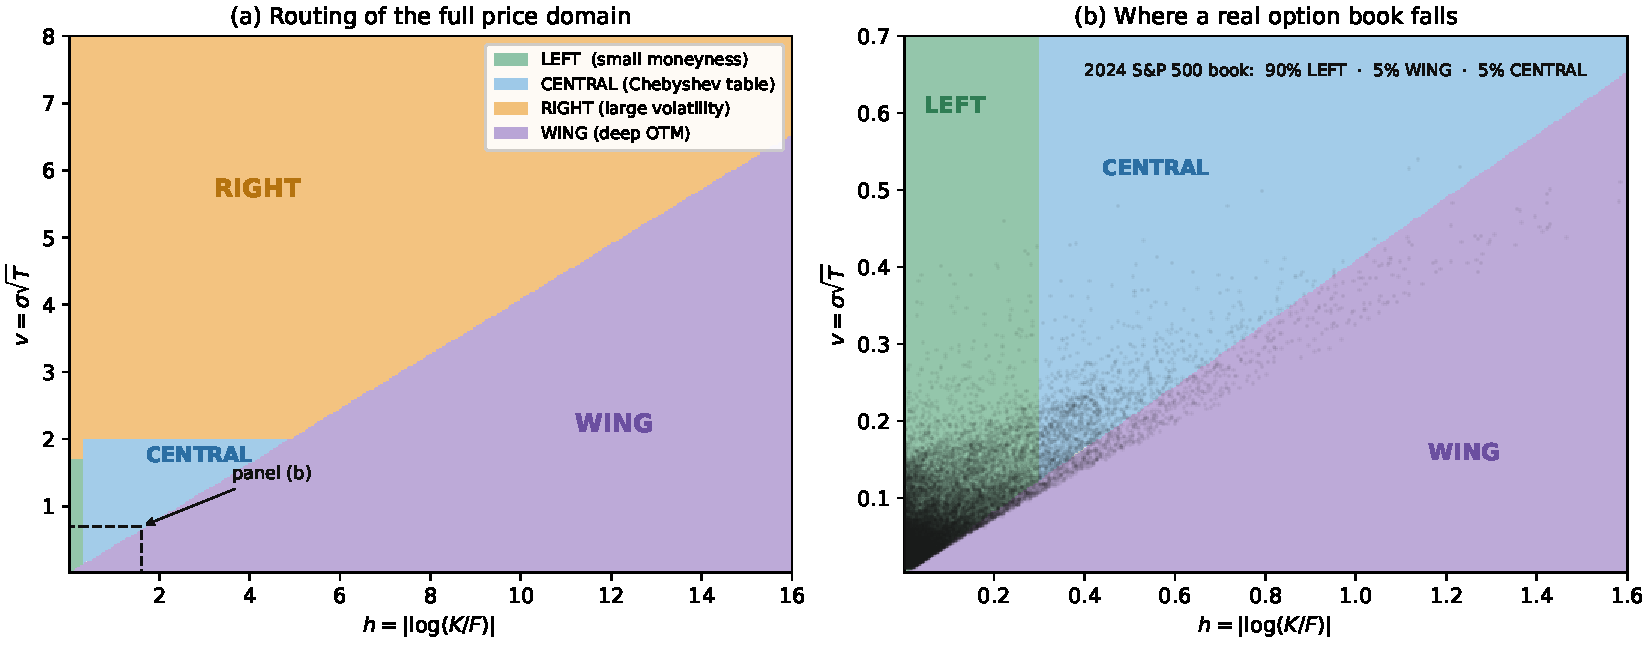
\includegraphics[width=\textwidth]{fig_routing_map}
\caption{Routing of the normalized price domain. \textbf{(a)} The feasible $(h,v)$ plane, $h=|\log(K/F)|$ and $v=\sigma\sqrt{T}$, partitioned into the four charts. The boundaries are fixed by the maturity-independent branch-point geometry of the inverse map, not tuned. \textbf{(b)} A zoom into the near-the-money corner (boxed in (a)) with an entire year of tradeable 2024 S\&P~500 end-of-day quotes overlaid. About $90\%$ of this book falls in the small-moneyness (LEFT) chart and a further $5\%$ in the deep wing, while the large-volatility (RIGHT) region that dominates the plane by area carries essentially none.}
\label{fig:routing}
\end{figure}

\subsection{The central table: \rtag{Central}}
\label{sec:table}

Over the interior of the domain the inversion is resolved by direct evaluation of a precomputed table, with no iteration at all. The rationale is a cost observation before it is an accuracy one. A machine-precision iterative inverter spends essentially all of its time in its accurate forward evaluations. A seed plus two Householder corrections costs two evaluations of a carefully written Black function, each dominated by error-function calls. A table evaluation replaces all of that by one polynomial sweep whose operation count is fixed, known at compile time, and free of data-dependent branches, which is also exactly the shape of computation that vectorizes. The questions that decide whether the approach reaches machine precision are which variable to tabulate, in which coordinate, and at what polynomial degree. All three answers come from the analytic structure of the inverse map.

The approximation target is the transformed variable $W$ of \eqref{eq:Wdef} rather than $\sigma$ or $w$ themselves. $W$ is the exponential scale variable of the wing asymptotics, it is nearly linear in $\log c$ across each cell, and fitting $\sigma$ directly was measured to cost one to two additional Chebyshev degrees per cell for no benefit. The abscissa is $\lambda=\log c$. The choice of $\lambda$ rests on a design principle about where the inverse map ceases to be analytic, which we state and then say precisely how far we have verified it. Viewed as a function of the price $c$ at fixed $h$, the inverse $w(h,\cdot)$ has branch points at the two endpoints $c=0$ and $c=1$, and the distances from an interior price $c$ to these branch points are exactly $c$ and $1-c$, \emph{independently of $h$}. The convergence of a Chebyshev approximation on a cell is governed by the Bernstein ellipse through the nearest \emph{complex} singularity \citep{trefethen2019approximation,masonhandscomb2003}. We have not proved that no complex singularity lies nearer than the two real endpoints, so we treat the endpoint distances as a predictive design principle and test it against the fitted degrees of all $181$ cells, where a nearer singularity would announce itself as degrees systematically above the prediction. The observed degrees match the prediction throughout (Figure~\ref{fig:branchgeom}). In the raw mantissa (binade) coordinate the $c=0$ branch point sits one octave to the left of every octave, in a self-similar way, which pins the Bernstein parameter at $\rho=3+2\sqrt2$ and predicts a floor of roughly twenty-one degrees per octave everywhere (confirmed by fits), so a transcendental-free table in that coordinate is a dead end, elegant as it looks. A conformal coordinate adapted to the annulus fares even worse in practice (fitted degrees near one hundred), because it compresses the real interval against the boundary. In $\lambda=\log c$ the distance to the branch point grows with the logarithmic cell width, and the fitted degrees fall to a median of ten, never exceeding sixteen. These are measured degrees from the table generator, not estimates.

\begin{figure}[t]
\centering
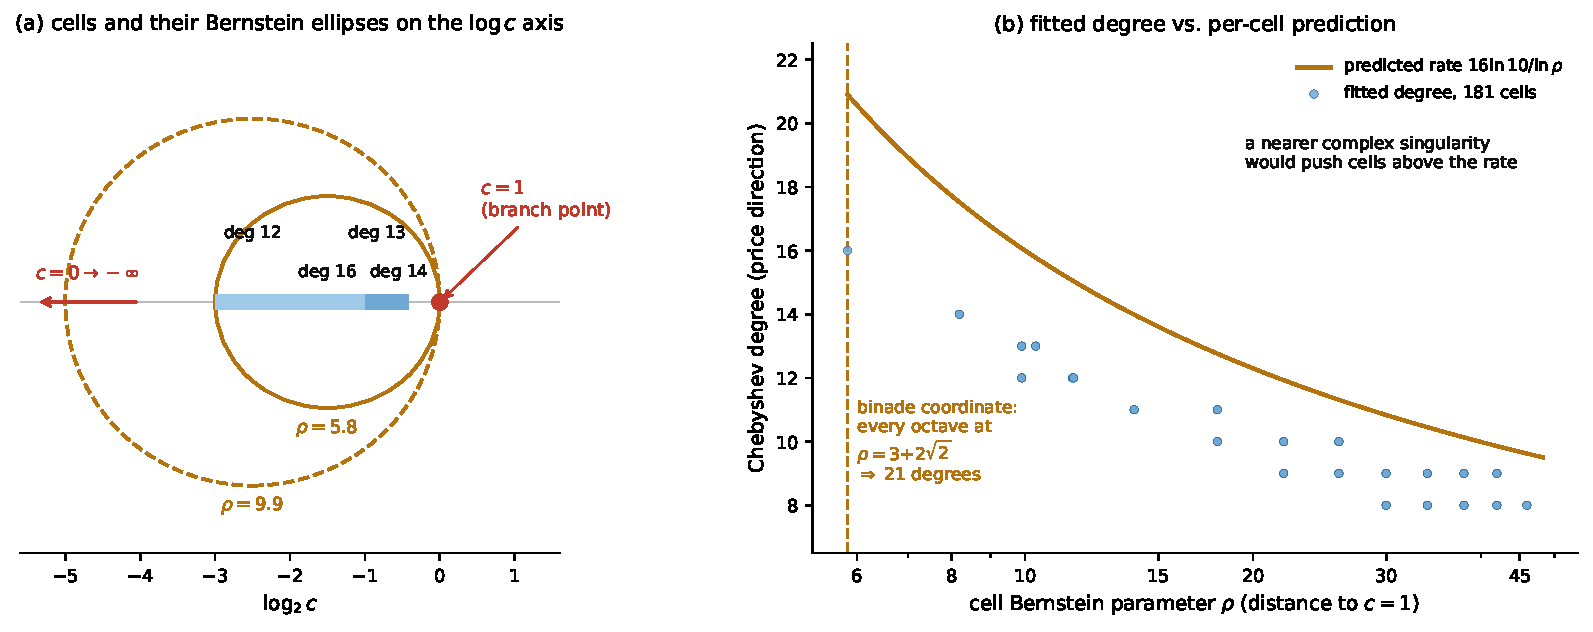
\includegraphics[width=\textwidth]{fig_branch_geometry}
\caption{The branch-point geometry that sizes the central table. \textbf{(a)} The cells nearest the money in one $h$-band of the shipped table, on the $\log_2 c$ axis, with the Bernstein ellipses of two of them drawn in place. Each cell's largest singularity-free ellipse passes exactly through the $c=1$ branch point, so the Bernstein parameter $\rho$ grows as cells recede from the money, while $c=0$ recedes to $-\infty$ in this coordinate. Without sub-splitting, the octave adjacent to the money would degenerate toward $\rho=1$. Sub-splitting those octaves (dark cells) together with the seam to the large-volatility chart keeps the worst normalized distance at $x=3$, the same worst case as the binade coordinate, so $\rho\ge3+2\sqrt2$ for every cell. \textbf{(b)} The fitted price-direction degrees of all $181$ cells against each cell's $\rho$, reconstructed from the shipped routing tables, with the predicted rate $16\ln10/\ln\rho$ overlaid. In the binade coordinate every octave sits at $\rho=3+2\sqrt2$ (dashed vertical), a flat floor of about twenty-one degrees. The fitted degrees track the predicted rate from below at a roughly uniform offset, the unknown order-one prefactor of the asymptotic rate. The endpoint distances remain a predictive design principle, not a proof that no complex singularity lies nearer. A nearer one would push cells systematically above the rate, and none appears.}
\label{fig:branchgeom}
\end{figure}

On each cell the table stores a bivariate Chebyshev surrogate
\begin{equation}
  W \;\approx\; \sum_{i=0}^{d_h}\sum_{j=0}^{d_\lambda} c_{ij}\,T_i(x_h)\,T_j(x_\lambda),
  \label{eq:cheb2}
\end{equation}
with $x_h,x_\lambda\in[-1,1]$ affine images of the local $h$-band and $\log c$ interval. The degree never exceeds sixteen in the price direction and thirteen in the moneyness direction, with median near ten. The full table comprises nineteen $h$-bands over $h\in[0.30,\,6.65]$ and $181$ cells holding about twenty-two thousand double-precision coefficients, just under $200$\,KB in total, small enough to be resident in a single core's L2 cache, so that in steady state the table costs no memory traffic. Cache-cold and cache-warm evaluation are indistinguishable after the first few hundred quotes of a batch, so residency is realized in practice. Recovery from the surrogate is the single map $w=h^2/(2W)$.

Routing to a cell is performed by integer operations on the IEEE-754 bit fields of the inputs, before any transcendental evaluation. The high bits of $h$ (exponent plus two leading mantissa bits) select the $h$-band. The exponent bits of $c$ select a price octave within the band, and the mantissa of $c$, forced into $[1,2)$, becomes the evaluation abscissa through the shared logarithm kernel of Section~\ref{sec:simd}, so that the per-quote classification involves no division, no logarithm and no comparison ladder. The octaves adjacent to $c=1$, where the near-at-the-money geometry would otherwise demand a special analytic branch, are instead refined by one or two additional mantissa bits into sub-cells, so that they become ordinary table cells. This sub-splitting is what removes the last analytic bypass from the interior.

The bands deliberately stop at $H_{\mathrm{box}}\approx6.65$. Beyond it the feasible strip is owned entirely by the endpoint charts of Sections~\ref{sec:left}--\ref{sec:wing}. For such large $h$ every feasible quote is either deep in the wing (small price) or above the $v=2$ seam (large volatility), so extending the table would add cells that no quote needs. The same reasoning caps the tabulated maturity range from below at $h=0.3$, where the matched small-moneyness chart is uniformly accurate. The table is therefore exactly as large as the region in which neither endpoint structure simplifies, and no larger.

The table is generated offline and oracle-gated before it is frozen. Chebyshev nodes for each cell are obtained by inverting exact double-precision prices with an arbitrary-precision solver at no fewer than twenty-five significant digits. The tensor coefficients are fitted, and the cell is accepted only if an \emph{independent} forty-digit oracle, distinct from the generator, confirms a relative $\sigma$ error below $10^{-15}$ on a dense sample of the cell including its boundaries. Cells failing the gate are re-fitted at higher degree or split. The same oracle-gated discipline applies to every auxiliary kernel of Section~\ref{sec:simd}.

\subsection{The small-moneyness chart: \rtag{Left}}
\label{sec:left}

For $h$ below the threshold $h<0.3$ the geometry collapses toward the explicit at-the-money line $c=\erf(\sigma/2\sqrt2)$: the level sets of $c$ crowd against an exactly known curve, and direct two-dimensional approximation of $w(h,c)$ degenerates precisely where the answer is simplest. The cure is a matched coordinate that absorbs the collapse. Scale the price by the leading $h$-dependence,
\begin{equation}
  \rho \;=\; \frac{c}{\expmone(h)},
\end{equation}
and let $A=B^{-1}(\rho)$ where
\begin{equation}
  B(A)\;=\;\frac{\varphi(A)}{A}-\PhiN(-A)\;=\;\int_A^\infty \varphi(u)\,u^{-2}\,\mathrm{d}u
\end{equation}
is an $h$-free, strictly decreasing universal function arising from the $t\to0$ layer of \eqref{eq:baseint}. The substitution $t=h/u$ maps the layer factor $e^{-h^2/(2t^2)}$ to the Gaussian $\varphi(u)$ and produces exactly the integral $B$, so the coordinate is dictated by the integral representation rather than chosen. The matched variable is $s=h/A$, which reduces to $v$ as $h\to0$, and in it the volatility has an even, regular expansion
\begin{equation}
  v(h,c) \;=\; v_0(\kappa s) + h^2V_2(s) + h^4V_4(s) + h^6 R(s,h),
  \label{eq:leftchart}
\end{equation}
where $v_0(\cdot)=2\sqrt2\,\erf^{-1}(\cdot)$ is the exact at-the-money kernel (the pair $(h,c)$ identifies the total standard deviation $v$, not the annualized $\sigma$, which only the convenience wrapper recovers as $\sigma=v/\sqrt T$), $\kappa=1/\sqrt{2\pi}$, and $V_2,V_4$ are elementary functions of $s$ alone. Evenness in $h$ is not an accident of fitting but the put--call symmetry $h\mapsto-h$ of the underlying density, and it is what makes the expansion efficient---each retained order gains a uniform factor $h^2$. This was verified directly, by halving $h$ at fixed $v$ and observing the residual error of the one-, two- and three-term truncations divide by $4$, $16$ and $64$. The leading term alone is uniformly second-order accurate through the deep-OTM corner (small $c$ jointly with small $h$) that defeats naive tabulation.

The chart is completed by two implementation decisions. First, the residual $R$ is small enough to be frozen once as a single low-order bivariate Chebyshev surface (degree two in the $h^2$ direction, sixteen in $s$). It absorbs everything beyond $h^4$ and brings the chart to machine precision across its whole strip. Second, the two functions $V_2$ and $V_4$, whose closed forms contain exponentials and a series crossover, are replaced by one-dimensional Chebyshev expansions in $s$ of degrees $28$ and $26$. This removes the last library call and the last data-dependent branch from the chart's inner loop, which matters for the vectorized path of Section~\ref{sec:simd}. The universal inverse $B^{-1}$ itself is evaluated by a three-regime branchless Chebyshev approximation, one regime in the variable $u=\kappa/(\rho+\tfrac12)$ for moderate arguments and two in $L=\log(1/\rho)$ for the tail, totalling $456$ bytes of coefficients with worst error $5.4\times10^{-16}$. The chain $c\mapsto\rho\mapsto A\mapsto s$ has relative condition number at most one, so no accuracy is lost in the transforms.

\subsection{The large-volatility chart: \rtag{Right}}
\label{sec:right}

At the opposite endpoint, $v>2$ and $c\to1$, the complement of \eqref{eq:baseint} is
\begin{equation}
  1-c \;=\; k\,e^{h/2}\int_v^\infty e^{-t^2/8}\,e^{-h^2/(2t^2)}\,\mathrm{d}t ,
\end{equation}
and the structural point that makes this endpoint fundamentally easier than the left one is that the layer factor is \emph{regular} there, with $e^{-h^2/(2t^2)}\to1$ as $t\to\infty$, with an expansion in $h^2/t^2$ that converges absolutely for every $t>0$. There is no layer to match, and termwise integration (justified by dominated convergence) yields an exact, absolutely convergent series rather than an asymptotic one. Introducing the ladder $B_n(A)=\int_A^\infty\varphi(u)\,u^{-2n}\,\mathrm{d}u$, which satisfies the elementary recursion $B_{n+1}(A)=\bigl[\varphi(A)A^{-(2n+1)}-B_n(A)\bigr]/(2n+1)$ with $B_0(A)=\PhiN(-A)$ and $B_1=B$, one obtains with $x=v/2$
\begin{equation}
  \frac{(1-c)\,e^{-h/2}}{2}
   \;=\; \PhiN(-x) + \sum_{n\ge1}\frac{(-h^2/8)^n}{n!}\,B_n(x).
  \label{eq:rightchart}
\end{equation}
Every identity in this subsection was checked against 30-digit arithmetic across the strip, with exact agreement to working precision.

Two consequences follow immediately. Setting $h=0$ in \eqref{eq:rightchart} identifies the leading inverse as the \emph{same} at-the-money kernel as on the left, evaluated at the transformed price
\begin{equation}
  \tilde c \;=\; 1-(1-c)\,e^{-h/2},
  \qquad
  v \;\approx\; 2\sqrt2\,\erf^{-1}(\tilde c)\;+\;h^2V_2^{R}+h^4V_4^{R}+\cdots,
\end{equation}
where $V_2^{R}=-B_1(x_0)/(4\varphi(x_0))$ and the higher coefficients are, through the ladder recursion, polynomials in $1/x_0$ and the Mills ratio $m(x)=\PhiN(-x)/\varphi(x)$. The Mills ratio is the only genuinely new one-dimensional function the endpoint requires. And since $B_n'(x)=-\varphi(x)x^{-2n}$, the series for the derivative of the right-hand side of \eqref{eq:rightchart} resums in closed form,
\begin{equation}
  g'(x) \;=\; -\varphi(x)\,e^{-h^2/(8x^2)} .
  \label{eq:gprime}
\end{equation}
The truncated ladder alone is excellent deep in the endpoint, where the expansion parameter $W=h^2/(2v^2)$ is small, but degrades toward moderate $v$. Table~\ref{tab:ladder} reports the verified relative error of the three-term truncation across the strip. The chart is therefore finished by iterating on \eqref{eq:rightchart} itself. The equation is exact and the derivative \eqref{eq:gprime} is cancellation-free and free of error functions. Moreover, because $\log|g'|$ is the elementary expression $\mathrm{const}-x^2/2-h^2/(8x^2)$, the higher derivative ratios needed by a third-order Householder step are closed-form rationals, $g''/g'=-x+h^2/(4x^3)$ and $g'''/g'=(g''/g')^2-1-3h^2/(4x^4)$, so an order-four step costs the same one price evaluation as a Newton step. This is the same economics that motivates Householder refinement in \citet{jackel2015rational}, and it halves the finisher: the implementation performs a \emph{fixed} count of three Householder steps with no early exit. The count was sized by measuring pure iteration convergence against exact prices. The seed degrades to a relative error of $0.27$ at the worst corner of the strip (near the wing seam, $W\approx3$), from which the fourth-order steps contract through $10^{-2}$, $10^{-7}$ and $10^{-27}$, so the third step lands with eleven orders of margin while two steps demonstrably do not suffice. A fixed count costs a little at benign points but buys determinism and lane-uniformity in the vectorized path. Prices above one half are handled throughout in the complement form, so that $1-c$ is never manufactured by subtraction. This, with the cancellation-free transform $c\mapsto\tilde c$, is why the chart retains full precision as $c\to1$ where a $\sqrt{FK}$-normalized formulation measurably does not (Section~\ref{sec:results}).

\begin{table}[t]
\centering
\small
\begin{tabular}{r r r r}
\toprule
$h$ & $v$ & $W=h^2/(2v^2)$ & rel.\ error of $V_0^{R}+h^2V_2^{R}+h^4V_4^{R}$ \\
\midrule
$0.3$ & $7.0$ & $0.0009$ & $1.8\times10^{-12}$ \\
$1.0$ & $7.0$ & $0.0102$ & $2.4\times10^{-9}$ \\
$2.0$ & $7.0$ & $0.0408$ & $1.5\times10^{-7}$ \\
$6.6$ & $7.0$ & $0.44$   & $1.7\times10^{-4}$ \\
$2.0$ & $2.5$ & $0.32$   & $2.0\times10^{-3}$ \\
\bottomrule
\end{tabular}
\caption{Verified relative accuracy of the three-term ladder seed of the large-volatility chart, before the Householder finisher. The expansion parameter is $W=h^2/(2v^2)$. The finisher's exact equation and closed-form derivatives bring every point to machine precision.}
\label{tab:ladder}
\end{table}

\subsection{The deep wing: \rtag{Wing}}
\label{sec:wing}

For prices below the table's reach the inversion works on the logarithm of the endpoint factorization of Section~\ref{sec:setup}, with the dominant asymptotic behaviour peeled off analytically. This is the extreme-strike regime whose leading-order asymptotics are classical (the moment formula of \citealt{lee2004moment}), but the chart must recover the map itself to full accuracy, not its leading order. Taking logarithms of $c=\gamma(h)e^{-W}W^{-3/2}H(W)$ turns the inversion into the implicit equation
\begin{equation}
  W \;=\; \widetilde L-\tfrac32\log W+\log H(W),
  \label{eq:wingeq}
\end{equation}
where $\widetilde L$ collects the price and $h$ data. Because the equation lives on the logarithm of the price, its conditioning is the benign $1/(2W)$ of Section~\ref{sec:setup}, and the inverter is validated on prices down to $10^{-320}$, that is, across the entire subnormal range of double precision. The shared logarithm kernel of Section~\ref{sec:simd} is extended by an exact power-of-two rescaling so that subnormal prices lose no accuracy on entry.

What makes the chart vectorizable is the evaluation of $\log H$. A runtime quadrature, the natural first implementation, has neither a fixed operation count in the useful sense (forty exponentials per evaluation) nor competitive speed, so it is retired to the offline oracle role and replaced by a frozen two-piece bivariate Chebyshev fit. The fitted quantity is deliberately not $\log H$ itself but the peeled, weighted residual
\begin{equation}
  S(u,\beta)\;=\;\frac{\log H}{u}+\Bigl(\beta+\frac32\Bigr),\qquad u=\frac1W.
\end{equation}
Peeling the leading asymptotic term $-(\beta+3/2)/W$ removes the dominant variation, and dividing by $u$ makes the fit's equioscillating error automatically proportional to the $\sigma$-tolerance, which grows like $W$. Fitting the raw residual instead was measured to demand degrees beyond thirty-six where the weighted form needs twenty-six. Two pieces with a generous overlap cover $W\in[2.5,\,260]$ ($668$ coefficients, $5.2$\,KB), the eight-term asymptotic series takes over beyond, and the piece-or-series regime is selected \emph{once} per quote from $\widetilde L$, so no per-step branching enters the kernel. The derivative $\partial_W\log H$ that drives the Newton steps is computed from the \emph{same} coefficients by the Chebyshev derivative recurrence, so the value and slope seen by the iteration are consistent by construction. The solve is a fixed count of six Newton steps. Five were originally de-risked on a sparse grid, and a dense sweep later exposed the choice as one step short at the high-$\beta$, low-$W$ corner, where convergence is slowest. Appendix~\ref{app:generation} records the incident. With six steps the chart passes the $10^{-15}$ oracle gate at every point of every feed, and it now shares the fixed-operation structure of the other charts, so the batch drivers evaluate it eight lanes at a time like the rest.

One boundary of the fitted table must be handled rather than clamped. The fit covers $\beta=h^2/16\le16.4$, i.e.\ $h\le16.2$, corresponding to strikes more than $10^{7}$ times the forward. Benchmark grids nevertheless reach past it, and a clamped evaluation there would return a plausible-looking volatility wrong in the third digit, the worst kind of failure. Quotes beyond the fitted $\beta$ therefore take a rare scalar branch. A seed obtained by dropping the second Black term and solving $\PhiN(v/2-h/v)=c$ in closed form (then restoring the dropped term by three fixed-point passes, worst seed error $0.23\%$ over $h\in[16.2,30]$), finished by the same three Householder steps as the warm-start entry. The branch is validated for $W\lesssim40$. The still-deeper corner, unreachable by any market data, returns a quiet NaN with an explicit out-of-domain status rather than a number (Section~\ref{sec:simd}). Both the scalar router and the batch drivers call the identical branch function, so the bit-identity invariant is preserved structurally.

\subsection{One family, analytically bounded, and derived seams}
\label{sec:unify}

A single identity ties the charts together. With
\begin{equation}
  H(W;a,\beta)\;=\;\int_0^\infty e^{-r}\Bigl(1+\frac rW\Bigr)^{-a}e^{-\beta/(W+r)}\,\mathrm{d}r,
\end{equation}
the substitution $u^2=A^2+2r$ gives, exactly,
\begin{equation}
  B_n(A)\;=\;\varphi(A)\,A^{-(2n+1)}\,H\!\Bigl(\frac{A^2}{2};\,n+\frac12,\,0\Bigr),
  \label{eq:unifyid}
\end{equation}
and the same family evaluated at $(a,\beta)=(3/2,h^2/16)$ and $(1/2,h^2/16)$ furnishes the two deep wings. Every special function appearing anywhere in the architecture is therefore one two-parameter family, and only two genuinely one-dimensional, $h$-independent inverses ($\erf^{-1}$ and $B^{-1}$) ever appear. In matched coordinates, all the $h$-dependence is a smooth prefactor times a regular even perturbation. For $\beta=0$ the family is Stieltjes,
\begin{equation}
  H(W;a,0)\;=\;\frac{1}{\Gamma(a)}\int_0^\infty\frac{t^{a-1}e^{-t}}{1+t/W}\,\mathrm{d}t,
\end{equation}
so its continued-fraction convergents bound it from alternating sides \citep{bakergravesmorris1996pade}, and $B$, every $B_n$, and by monotone inversion $B^{-1}$ admit rigorous two-sided enclosures at any order (the one place the word \emph{certified} applies in its strict sense), and these enclosures supply the truth values against which the endpoint kernels were gated. For $\beta>0$ the Stieltjes property fails (the Borel transform of the wing series changes sign, and the Herglotz--Pick criterion is violated numerically), but the exact identity $H(W;a,\beta)=H(W;a,0)-\int_0^\infty\!\sqrt{\beta/\tau}\,J_1(2\sqrt{\beta\tau})\, e^{-W\tau}\,H(W(1{+}\tau);a,0)/(1{+}\tau)\,\mathrm{d}\tau$, obtained by writing $1-e^{-\beta s}$ as the classical $J_1$ Laplace transform \citep[Ch.~10]{olver2010nist} and applying it under the integral sign, expresses $H(\cdot\,;a,\beta)$ through the $\beta=0$ family (we exercise it numerically to $10^{-21}$ in the generation pipeline), so two-sided enclosures extend to the wing evaluators as well.

The seams between the charts are derived, not tuned. The truncation error envelopes of the two endpoint expansions follow the scaling laws (asymptotically motivated, confirmed by high-precision measurement of the envelopes) $E_{\mathrm{left}}\propto v^2h^{2N+2}$ and $E_{\mathrm{right}}\propto\bigl(h^2/2v^3\bigr)^{N+1}$, and equating envelopes across the wide overlap bands, where two charts are simultaneously accurate, yields thresholds that are constants in the matched coordinates. The implementation freezes all three as one-dimensional price curves, each a single Chebyshev polynomial in $h$: the wing seam $c_{\mathrm{wing}}(h)=C(h,h/\sqrt6)$ (the level set $W=3$), the central--right seam $c_2(h)=C(h,2)$ (the level set $v=2$), and, within the small-$h$ band, the left--right seam $c_{\mathrm{tl}}(h)=C(h,1.70)$, placed at $v=1.70$ rather than $v=2$ so that the exact-equation Householder refinement of Section~\ref{sec:right}, rather than an extrapolated finisher, owns the corner where the two charts meet. Freezing the seams as polynomials matters beyond tidiness. Routing then costs three short polynomial sweeps rather than any runtime price evaluation, which is what allows the classification itself to vectorize (Section~\ref{sec:simd}). A fitted seam differs from the exact boundary only within its fit error ($\sim10^{-16}$ relative), reclassifying at most quotes within a ulp of the seam---inside the overlap bands, where both neighbouring charts are machine-precise, so nothing delicate happens at a crossing. The dense seam sampling reported in Section~\ref{sec:results} confirms it.

The resulting coverage map is this. The deep wing owns $W\gtrsim3$, including the feasibility pinch at very large $h$, which is a wing region in disguise since the feasible price there is necessarily small. The small-moneyness chart owns $h<0.3$ up to the $v=1.70$ seam. The large-volatility chart owns everything above its seam, including the whole strip $h>H_{\mathrm{box}}$ that is not wing. The central table owns the remainder. The four regimes tile the domain exactly, and on a broad random feed no feasible quote fails to route.

\paragraph{The accurate forward.}
As in \citet{jackel2015rational}, the precision floor of the whole method is the accuracy of the forward evaluation used inside the places that refine, the large-volatility Householder finisher and the warm-start entry of Section~\ref{sec:simd}. We evaluate the normal functions there through a scaled complementary error function $\erfcx$ built on frozen Chebyshev pieces in the spirit of \citet{cody1969rational}, three degree-$22$ pieces covering $[0,7.2]$, selected per lane by blends off the critical path, which halves the sequential Clenshaw chain relative to a single degree-$36$ fit and extends the domain to the arguments the warm-start basin requires, and an exponential reduced by a Cody--Waite splitting of $\log2$ followed by a Chebyshev polynomial on $[-\tfrac12\log2,\tfrac12\log2]$ and an exact power-of-two scaling. Both Black terms of a price residual are produced by one shared kernel that evaluates the $\pm$ pair from a single $\erfcx$ core and one shared normal tail, with a compensated square killing the rounding of the squared argument, so each refinement step costs two $\erfcx$ and four exponential evaluations rather than the naive six. The refiners therefore perform no library $\erf$, $\erfc$ or $\exp$ call, their rounding behaviour is fully determined by the frozen coefficients, and the rational quantile seed's $10^{-9}$ error is immaterial because the equation being solved is exact.

\section{Routing and the bit-identical vectorized implementation}
\label{sec:simd}

This section develops the runtime phase sketched in Algorithm~\ref{alg:overview}, namely how each quote is routed into its regime and evaluated by kernels the scalar and SIMD paths share bit-for-bit. The offline generation is detailed in Appendix~\ref{app:generation} and the per-chart kernels in Appendix~\ref{app:hotpath}.

The design goal that shapes the implementation is that a batched evaluation must return, for every quote, the same double-precision result as the scalar entry point, bit for bit. This is not a convenience. It means the vectorized surface and grid drivers can be validated by the single statement ``batch equals scalar'', and it removes any possibility that the fast path and the reference path silently disagree. The invariant is achieved by writing every kernel as a branchless chain of \emph{explicitly ordered} fused multiply--adds and sharing that exact code between the scalar and SIMD paths.

Three kernels are shared. A branchless logarithm proxy evaluates $\log_2 m$ for a mantissa $m\in[1,2)$ through the reduction $t=(m-1)/(m+1)$ and a Chebyshev series in $t^2$, with absolute error a few units in the last place, comparable to the library function it replaces. A full natural logarithm, needed by the universal inverse, the quantile seed and the wing, is then assembled by reuse as $\log x=\log2\,(e+\log_2 m)$ from the exponent $e$ and mantissa of $x$, introducing no new approximation and agreeing with the library logarithm to three units in the last place over the domains that consume it. A subnormal-safe variant rescales arguments below the normal range by an exact power of two before the bit extraction, so the wing's prices near $10^{-320}$ enter with full accuracy. A degree-seventeen branchless kernel evaluates the at-the-money base $v_0=2\sqrt2\,\erf^{-1}$. And a bivariate Chebyshev evaluator computes \eqref{eq:cheb2} by an inner accumulation in $x_\lambda$ followed by an outer Clenshaw sweep in $x_h$. One design lesson from gating these kernels deserves record, because it is counterintuitive. For a kernel that feeds a downstream polynomial fit, the smoothness of its error function matters as much as its magnitude. An early candidate for the logarithm kernel, a plain minimax polynomial of the \emph{same} worst-case accuracy as the reduction above, raised the Chebyshev degrees demanded by the table cells by eleven, because its equioscillating error injected a rough component into the quantity being fitted. The smooth-error reduction adds no degree at all. Kernel acceptance was therefore gated on the downstream fitted degrees, not only on the kernel's own error.

Each kernel has an eight-wide AVX-512 twin and a four-wide AVX2 twin that reproduce the scalar fused-multiply order lane for lane. Masked selections use blends whose argument order is mirrored from the scalar ternaries, and per-lane routing decisions are the same integer tests as the scalar router. The only intrinsic without a direct AVX2 analogue is the exponent scaling $\mathtt{scalef}$ used by the shared exponential. We reproduce it, including its behaviour in the subnormal underflow range, by an exact two-factor power-of-two construction (splitting the integer exponent so that each factor remains a normal number), so the AVX2 path matches both the scalar $\mathtt{ldexp}$ and the AVX-512 $\mathtt{scalef}$ across the whole finite range. The equivalence was verified bit-for-bit over seven hundred thousand arguments down to the underflow threshold.

The batch driver is shaped by what a real workload contains. An end-of-day option book, re-expressed on the out-of-the-money branch (Section~\ref{sec:results}), is about $90\%$ small-moneyness quotes. A general mixed-maturity batch is therefore dominated by one chart, and the driver bets on that. It streams the $(h,c)$ vector eight (or four) lanes at a time and, for each block, does three things at once. It classifies every lane by evaluating the three seam curves. It evaluates the small-moneyness kernel on \emph{every} lane speculatively, and it stores, with a masked write, only the lanes that classified as small-moneyness. Those are the $\sim\!90\%$, written in input order with no sort and no scatter. The minority that classified otherwise is compressed into a small deferred buffer and handed to a conventional counting-sort-by-cell pass over the remaining charts. Because the dominant chart never touches the sort, the mixed-maturity cost per quote falls close to the kernel's own cost rather than to the cost of routing plus sorting plus gathering every quote individually.

Making the classification itself vectorizable required removing the last library calls from the router. The two seam prices consumed on the hot path, $C(h,1.70)$ (small-moneyness versus large-volatility) and $\expmone(h)$ (the small-moneyness input), are replaced by frozen low-degree Chebyshev fits, and the wing and central seams are moved onto the shared $\exp$ kernel. The scalar entry adopts the identical fits, so the classification is a handful of branchless polynomials that the scalar and SIMD routers evaluate to the same bits, and the route each quote takes is unchanged. Speculation costs the wasted small-moneyness evaluations on the deferred minority, far less than the sorting it removes on the majority, and it is gated. A strided sample of the batch's moneyness picks the speculative driver only when the small-moneyness share is actually high, and otherwise falls back to the plain counting-sort-by-cell driver, which is faster on the wing- or central-dominated feeds a real book never produces. Both drivers return bit-identical results, so the dispatch changes only speed.

Three further drivers complete the set. A fixed-moneyness batch driver for the case in which all quotes share one $h$ (so the $h$-derived constants are hoisted out of the loop entirely) is the throughput ceiling. Note that this is a fixed-moneyness batch, not an expiry slice, since at one maturity $h$ varies across strikes. A permuted-output variant returns results in bucket order with the permutation, saving the scattered store when the caller can consume sorted output. And a warm-start driver for streaming recalibration takes the previous variance of each $(K,T)$ node as its seed, skips routing entirely, and applies three fixed Householder steps on the exact equation. Within its basin (previous $W\le40$, volatility moving up to a few percent) it returns the new root to within a few ULP rather than the last bit, because the half-ULP rounding of its working variables is amplified by the deep-wing cancellation ratio, so a caller needing full accuracy re-inverts cold---a documented API contract. For the live streaming regime, where snapshot-to-snapshot moves are sub-percent, a measured two-step variant reaches the same warm floor as three steps (verified for $|\Delta v/v|\le1\%$ at every $W\le40$. It degrades only from $2\%$ moves at deep $W$) and is guarded by the size of its own last correction, so a move outside the two-step basin flags itself and falls back to a cold inversion rather than returning a degraded result silently. A thin book-mode wrapper packages the pattern. Exchange strike grids are standardized, so a live book's $(K,T)$ node set is persistent, the caller carries only static log-strikes and previous variances, and re-deriving $h$ under a new forward is one subtraction per node before the whole book warm-refines with no routing at all. In every driver the deep-wing bucket is split by the wing's three evaluation regimes so each sub-bucket is lane-uniform, and the wing kernel has both an AVX-512 and an AVX2 twin. Two routes remain scalar by design. The exact at-the-money line $h=0$ and the rare large-$\beta$ rescue branch of Section~\ref{sec:wing}. Both drop to the same non-inlined scalar entry the reference path uses, so the bit-identity statement covers them trivially.

The correctness of the vectorization is checked adversarially rather than assumed. Perturbing a single constant inside the vector kernels alone, by one part in $2^{40}$, makes the batch result diverge from the scalar result on precisely the quotes routed through those kernels, while the unperturbed build shows zero divergences. This confirms the vector path genuinely executes rather than silently falling back to the scalar kernels and passing the identity check vacuously. The same check was run independently for the AVX-512 and AVX2 builds.

The bit-identity invariant turns out to constrain the \emph{build}, not only the source, and the constraint is instructive enough to record as a finding. Under GCC's default C\raise.08ex\hbox{\tt ++} contraction mode (\texttt{-ffp-contract=fast}) the compiler is free to fuse any multiply--add pair into a single fused operation with one rounding \citep{ieee754_2019,muller2018handbook,goldberg1991floating}, and it exercises that freedom during middle-end optimization, \emph{after} inlining, so which pairs fuse depends on the inlining context of the surrounding translation unit. We observed the same header, compiled at identical flags into two translation units of one program, produce two floating-point functions that disagree by one to five ULP on about seven percent of deep-wing quotes. A non-inlined entry point compiled to $4{,}427$ instructions in the benchmark unit and $2{,}932$ in a test unit, from identical source. Source-level care does not defend against this, because the divergence is the optimizer's context-dependent choice. The robust discipline is the opposite default---contraction \emph{off}, every intended fusion an explicit $\operatorname{fma}$. Since the accuracy-critical chains here were written that way from the start, the flag costs nothing measurable, and it upgrades determinism from a per-build property to a portable one. Bitwise-reproducible floating point has mostly been pursued for reductions, where reassociation is the hazard \citep{demmel2015reproducible}. The discipline here targets the complementary hazard, fusion, to the same end. On every validation feed of Section~\ref{sec:results}, the AVX-512, AVX2 and non-SIMD builds, compiled with either GCC~11 or Clang~14, return bitwise-identical doubles for every quote, scalar and batch paths alike, verified by byte comparison of the full output vectors, not by summary statistics. In production terms, a risk system replaying a batch or reconciling results across heterogeneous nodes and compilers obtains identical doubles in every case, removing a class of reconciliation noise that solvers with data-dependent iteration counts can exhibit.

\paragraph{The input contract.}
A reference implementation is defined as much by what it does with bad inputs as by its accuracy on good ones, because a live feed delivers crossed quotes, stale prices and convention violations as a matter of course, and the worst possible response is a plausible-looking number. The entry points therefore implement a \emph{total} contract: every representable pair $(h,c)$ returns either a machine-precision result or a quiet NaN, and a checked variant reports a machine-readable status alongside, at or below intrinsic ($c\le0$), at or above the forward bound ($c\ge1$), convention violation ($h<0$ or NaN input), the out-of-domain deep corner of Section~\ref{sec:wing}, and a near-saturation advisory for $v>8$, where the $1-c$ representability bound of Section~\ref{sec:setup} limits what any double-precision inverter can resolve. In that last case the best-effort result is still returned. A convenience wrapper accepts the industry-convention inputs (forward, strike, undiscounted price, expiry, call/put flag), performs the in-the-money to out-of-the-money parity flip internally, and returns the annualized volatility with the same status, which removes the most common integration error, a wrong normalization, from the caller's responsibility.

\section{Numerical results}
\label{sec:results}

\paragraph{Oracle and test sets.}
The reference is an independent \texttt{mpmath} inverter at 40 significant digits that inverts the given double-precision price $c$ by a bounded log-space Newton iteration (not \texttt{findroot}, not a round trip). Accuracy is the relative error $|\hat\sigma-\sigma_{\text{oracle}}|/\sigma_{\text{oracle}}$, and we also report the worst-case error in units in the last place (ULP) of double precision. We score on a $150\times110$ grid over $h\in[0.02,16]$, $\sigma\sqrt T\in[0.02,8]$ ($16{,}039$ feasible points, the ``regular'' set), on a hand-built ``stressed'' set of deep-wing, near-intrinsic and small-$h$ deep-OTM points, and on a $3{,}511$-point chart-stress feed constructed to exercise every routing region and seam. The competitor is the latest public C\raise.08ex\hbox{\tt ++} implementation of \citet{jackel2015rational}, downloaded unmodified from the author's website (Appendix~\ref{app:artifacts}), called through its normalized entry point with $\beta=c\,e^{-h/2}$. We verified on the extreme cases that this normalized call agrees with the library's direct price interface, so no artefact of the calling convention enters the comparison. Per the scoring rule of Section~\ref{sec:setup}, no method is scored against the volatility that \emph{generated} a test price. On our feeds that round-trip construction error reaches tens to hundreds of ULP in the wings, identically for all methods tested. All figures below are free of it.

\paragraph{Hardware, compilers and timing protocol.}
All measurements were taken on an Intel Core i5-1145G7 (Tiger Lake, AVX-512-capable, four cores) under Linux (Ubuntu 22.04, WSL2), with GCC~11.4 at \texttt{-O3 -ffp-contract=off -fno-fast-math} and the instruction set selected per build (\texttt{-march=native} for AVX-512, \texttt{-mavx2 -mfma -mno-avx512f} for AVX2, both SIMD sets disabled for the scalar build). The Clang~14 cross-check uses the same flags. The timing protocol guards against dead-code elimination with a volatile accumulator. The definitive figures of Table~\ref{tab:timing} come from the same machine quiesced (mains power, no concurrent load, the process pinned to a fixed core), running each benchmark binary five times, each internal row itself a median over fifteen timing passes of eight repeats. The table reports medians across the five executions, whose spread is under one percent. Contraction is disabled for the reproducibility reasons of Section~\ref{sec:simd} (every intended fusion is an explicit $\operatorname{fma}$), and \texttt{-ffast-math} is deliberately avoided because it would break the scalar/SIMD bit-identity. The floating-point environment is the IEEE-754 default: round-to-nearest-even, gradual underflow (no FTZ/DAZ), hardware $\operatorname{fma}$. Bit-identity is claimed for the tested configurations (two compilers by three instruction-set builds on this host), not for arbitrary hardware. The development host is a virtualized laptop, so only the quiesced, pinned protocol above produces reported numbers.

\begin{table}[t]
\centering
\small
\begin{tabular}{l r r r r r r}
\toprule
 & \multicolumn{3}{c}{Routed table inverter} & \multicolumn{3}{c}{Let's Be Rational} \\
\cmidrule(lr){2-4}\cmidrule(lr){5-7}
Region & max rel & RMS rel & max ULP & max rel & RMS rel & max ULP \\
\midrule
Central          & $4.3\times10^{-16}$ & $1.2\times10^{-16}$ & 3 & $5.0\times10^{-16}$ & $1.2\times10^{-16}$ & 3 \\
Left (small $h$) & $6.7\times10^{-16}$ & $2.3\times10^{-16}$ & 4 & $8.3\times10^{-16}$ & $2.4\times10^{-16}$ & 5 \\
Right (large $v$)& $4.3\times10^{-16}$ & $1.0\times10^{-16}$ & 3 & $1.1\times10^{-13}$ & $4.8\times10^{-15}$ & 867 \\
Wing (deep OTM)  & $7.9\times10^{-16}$ & $9.6\times10^{-17}$ & 5 & \multicolumn{3}{c}{degrades, see text} \\
\midrule
All              & $\mathbf{7.9\times10^{-16}}$ & $1.0\times10^{-16}$ & $\mathbf{5}$ & --- & --- & --- \\
\bottomrule
\end{tabular}
\caption{Relative error in $\sigma$ against a 40-digit oracle on the regular set ($16{,}039$ points). The routed inverter has \emph{no} point above $10^{-15}$. Its worst error is $7.9\times10^{-16}$ ($5$ ULP). Let's Be Rational matches it on the central and small-$h$ regions but degrades in the near-intrinsic right endpoint and the deep wing (text).}
\label{tab:accuracy}
\end{table}

\paragraph{Accuracy.}
Table~\ref{tab:accuracy} and Figure~\ref{fig:heat} give the result. The routed inverter holds below $10^{-15}$ at \emph{every} point of the feasible domain, with a worst relative error of $7.9\times10^{-16}$ (5 ULP) and a median at the level of a single rounding. On the interior and the small-$h$ region it is indistinguishable from Let's Be Rational, confirming that the table construction reaches the same last-bit accuracy as a state-of-the-art iterative solver. The two methods separate only at the extremes (Figure~\ref{fig:errorprofile}). In the near-intrinsic right endpoint ($c\to1$, $\sigma\sqrt T\to8$) the reference solver loses up to $867$ ULP where the routed inverter stays at $3$ ULP, because the cancellation-free transformed price $\tilde c$ of Section~\ref{sec:right} avoids the loss that $1-c$ incurs. In the deep wing the two methods receive inputs of different quality. The reference's $\sqrt{FK}$-normalized price $\beta=c\,e^{-h/2}$ is smaller than the forward-normalized $c$ by the factor $e^{-h/2}$, so at large $h$ it reaches the subnormal range, where doubles carry fewer significant bits, several hundred orders of magnitude before $c$ does. Its accuracy there reflects that input conditioning rather than its iteration. The routed inverter, whose wing chart works on the logarithm of the intact price, inverts prices down to $10^{-320}$ at machine precision. The stressed set tells the same story, with $0$ routed points above $10^{-15}$ (worst $6.9\times10^{-16}$) against a $3.4\times10^{-14}$ right-endpoint tail for the reference. Across all validation feeds combined, including the chart-stress feed, the worst error the routed inverter has exhibited anywhere is $8.3\times10^{-16}$. No feed has produced a point above $10^{-15}$. The seam crossings between charts were additionally sampled densely on both sides. No error excursion occurs at any of them. This was not automatic. Dense seam verification exposed two seam placements whose corners violated the gate, and both were corrected (one by moving the small-$h$ left--right seam to $v=1.70$, one by extending the wing crossover), the intended operation of an oracle-gated design.

Honesty about where the accuracy advantage does and does not matter is essential here. The two regimes in which the reference degrades---the near-intrinsic upper endpoint and the subnormal-price wing---are extreme. They require normalized prices within a rounding of one, or below $10^{-40}$. A tradeable option book reaches neither. Inverting an independent $30$-digit oracle on $1{,}150$ \emph{actual} projected prices sampled from the 2024 S\&P~500 book (described below), stratified to over-weight the deep-cheap and seam-band quotes, the routed inverter has no point above $10^{-15}$ (worst $8.5\times10^{-16}$), and so does the reference. On real market data, in other words, both solvers are at machine precision, and the case for the present method there rests on throughput and determinism, not on accuracy. The accuracy advantage is real but it is insurance. It guarantees the same last-bit behaviour on the theoretical, stressed, and finer-tick inputs that a robust production system must also survive, without the reference's two localized failure modes.

\begin{figure}[t]
\centering
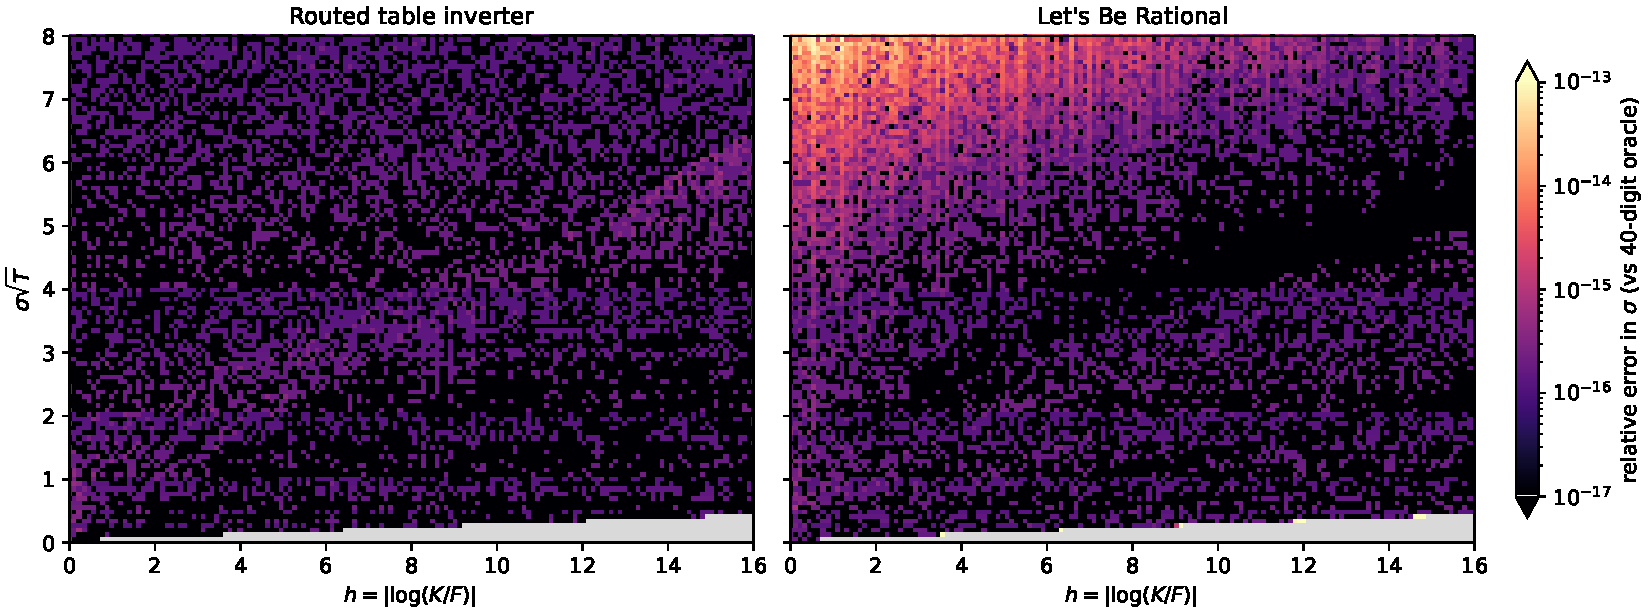
\includegraphics[width=\textwidth]{fig_accuracy_heatmap}
\caption{Relative error in $\sigma$ against the 40-digit oracle over the $(h,\sigma\sqrt T)$ domain. The routed table inverter (left) is uniformly at machine precision. Let's Be Rational (right) degrades in the near-intrinsic upper-left corner and, more mildly, in the deep wing. Grey marks prices that round to $0$ or $1$ in double precision.}
\label{fig:heat}
\end{figure}

\begin{figure}[t]
\centering
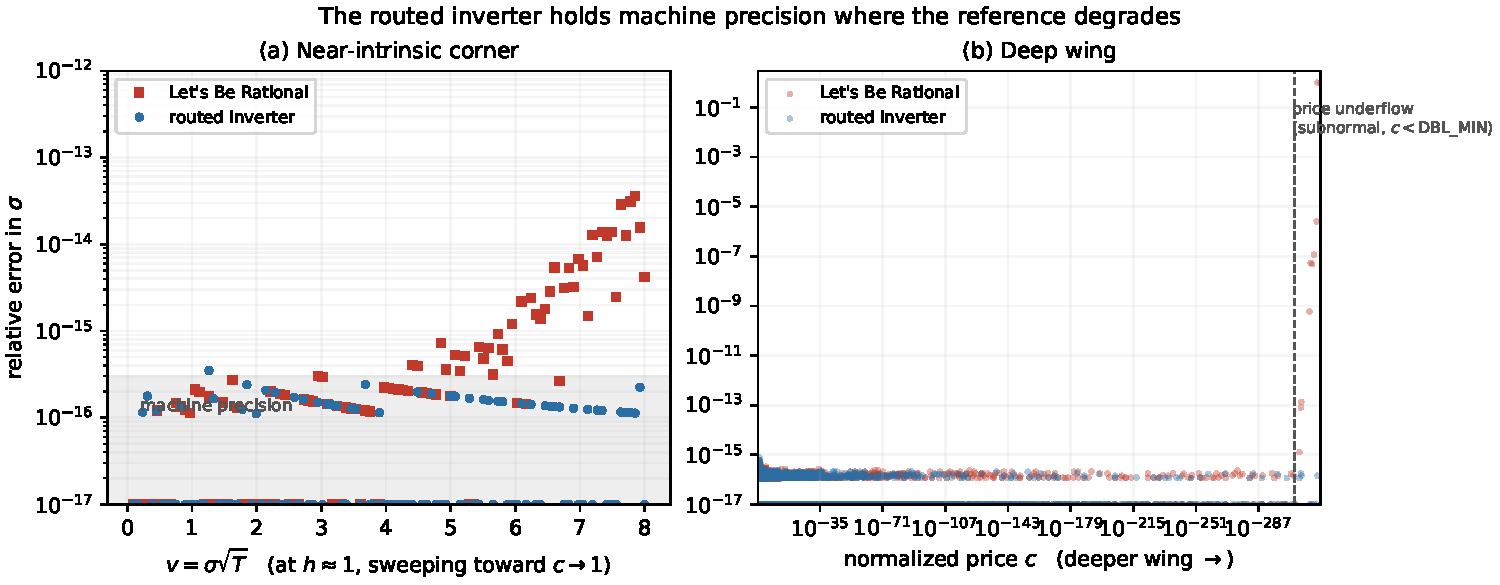
\includegraphics[width=\textwidth]{fig_error_profile}
\caption{Relative error in $\sigma$ against the $40$-digit oracle in the two regimes where the reference degrades. \textbf{(a)} Near the intrinsic value: at fixed $h\approx1$, as $v$ grows and the normalized price $c\to1$, Let's Be Rational climbs toward $10^{-13}$ from the $1-c$ cancellation while the routed inverter stays at machine precision. \textbf{(b)} In the deep wing, error against the price magnitude $c$ over the whole wing chart. Both solvers hold machine precision across three hundred orders of magnitude, but once the price is subnormal ($c<\mathrm{DBL\_MIN}$) the reference's reduced variable $\beta=c\,e^{-h/2}$ underflows and it loses precision, whereas the routed inverter, working in $c=\text{price}/F$, does not.}
\label{fig:errorprofile}
\end{figure}

\paragraph{Edge cases.}
Table~\ref{tab:edge} isolates individual extreme inputs, with the exact double-precision price each method was given and the relative $\sigma$ error each returned. The routed inverter is exact or within four ULP on every row, including prices in the subnormal range near $10^{-321}$, the formerly excluded small-$h$ deep-OTM corner, the near-intrinsic upper endpoint, and the feasibility pinch at $h=16$. The reference solver's two visible losses have different characters and should be read differently. Near the intrinsic value its error ($10^{-14}$ scale) is algorithmic, the cancellation discussed in Section~\ref{sec:setup}. In the subnormal wing its input $\beta=c\,e^{-h/2}$ has already lost significance before the algorithm starts, so the error there ($10^{-6}$ to $10^{-4}$) reflects the conditioning of its chosen normalization rather than its iteration. The routed inverter is immune because its normalization keeps the small price intact and its wing chart works on the logarithm of the price. At the two most extreme prices of the regular grid, below $10^{-320}$, the $\beta$ input underflows to exactly zero and the reference necessarily returns zero volatility, while the routed inverter still recovers $\sigma$ to the correctly rounded last bit. Prices this small are admittedly of more diagnostic than trading interest, but they mark where each formulation's validity actually ends.

\begin{table}[t]
\centering
\small
\begin{tabular}{r r l l r r}
\toprule
$h$ & $\sigma\sqrt T$ & price & regime & \multicolumn{1}{c}{this method} & \multicolumn{1}{c}{Let's Be Rational} \\
\midrule
$14.8$  & $0.386$  & $c=9.9\times10^{-321}$    & wing   & $0$                  & $1.4\times10^{-4}$ \\
$3.56$  & $0.0932$ & $c=2.2\times10^{-321}$    & wing   & $0$                  & $3.9\times10^{-6}$ \\
$8$     & $0.90$   & $c=1.5\times10^{-18}$     & wing   & $1.2\times10^{-16}$  & $0$ \\
$0.29$  & $0.02$   & $c=9.6\times10^{-51}$     & corner & $0$                  & $0$ \\
$10^{-4}$ & $1.0$  & $c=0.38$                  & left   & $0$                  & $0$ \\
$0$     & $6.4$    & $c=0.9986$                & ATM    & $5.6\times10^{-16}$  & $1.4\times10^{-16}$ \\
$0.5$   & $7.9$    & $1-c=1.0\times10^{-4}$    & right  & $1.1\times10^{-16}$  & $5.6\times10^{-16}$ \\
$1.2$   & $7.93$   & $1-c=1.3\times10^{-4}$    & right  & $1.1\times10^{-16}$  & $1.3\times10^{-14}$ \\
$16$    & $7.5$    & $c=0.93$                  & right  & $1.2\times10^{-16}$  & $1.2\times10^{-16}$ \\
\bottomrule
\end{tabular}
\caption{Relative error in $\sigma$ against the 40-digit oracle on hand-picked extreme inputs. An entry of $0$ means the returned double equals the correctly rounded oracle value. The reference solver's subnormal-wing losses reflect the conditioning of its $\sqrt{FK}$ normalization (text). Its near-intrinsic losses arise in its own normalized variable near the upper price bound, where its objective conditions poorly---an observed property of that implementation, distinct from the representability bound of Section~\ref{sec:setup}, which binds both methods equally.}
\label{tab:edge}
\end{table}

\paragraph{Coverage and bit-identity.}
On a broad random feed of $120{,}000$ quotes ($\sigma\sqrt T$ up to $8$, $h$ up to $16.5$) every quote routes to a chart and returns a gated result, with no routing failures and no silent fallbacks. The continuum contract remains the graded one of Section~\ref{sec:setup}. Across the scalar, AVX2 and AVX-512 builds and all batch drivers (fixed-$h$ batch, mixed-$h$ grid, permuted-output, warm-start), the batch result equals the scalar result on every one of the $120{,}000$ quotes, with zero mismatches. The same holds on the $16{,}039$-point accuracy grid. Beyond within-build identity, the full output vectors of the three instruction-set builds under GCC and of the AVX-512 and AVX2 builds under Clang were compared byte for byte on the chart-stress feed: all five binaries return identical doubles for every quote, in both the scalar and the batched path. The accuracy of Table~\ref{tab:accuracy} is therefore simultaneously the accuracy of every batch path, every instruction set, and both compilers.

\paragraph{What a real book exercises.}
Which charts does a realistic workload actually hit? We took one full year (2024) of end-of-day S\&P~500 index option quotes from a standard vendor file ($1.85$ million with positive volume and open interest), and applied a tradeability screen: a live, uncrossed two-sided market, mid price at least five cents, relative bid--ask spread at most $25\%$, open interest at least $100$ contracts and volume at least $10$, and at least a week to expiry. This leaves $641{,}072$ tradeable quotes. Forwards are the vendor's own, matched to each quote by expiry \emph{and} settlement convention (the file carries distinct AM- and PM-settlement forwards, differing by about half an index point), and discount factors come from the vendor zero curve. We do not rely on a parity regression, which we found can bias the implied forward by up to several tenths of a percent at individual expiries where deep in-the-money premiums dominate the fit. Every surviving quote (call or put, in- or out-of-the-money) is then folded onto the single out-of-the-money-call branch by put--call parity, exactly the reduction the inverter itself uses. $15.8\%$ of quotes are in-the-money and reach the branch through the parity projection. Routing the resulting $(h,c)$ pairs gives: small-moneyness chart $90.0\%$, deep wing $5.1\%$, central table $4.9\%$, large-volatility chart $0.0\%$ (Figure~\ref{fig:routing}). Three facts deserve emphasis. The wing, though a single-digit fraction, is a permanent feature of this book---one tradeable quote in twenty, $98\%$ of them downside puts, the crash-skew tail \citep{hagan2002smile} firing the wing route on absolute cheapness---which is what motivated vectorizing it rather than leaving it scalar. The large-volatility chart never fires on end-of-day equity-index data. It earns its place as coverage, not throughput. And the maximum log-moneyness observed all year is $h=3.4$, far inside the design domain. The uniform broad box used for coverage stress, by contrast, is $78\%$ wing---a distribution no traded book resembles---so throughput is reported on a market-realistic feed, built by resampling $30{,}000$ quotes from this tradeable population, which reproduces the live route mix.

\paragraph{Throughput.}
Table~\ref{tab:timing} and Figure~\ref{fig:throughput} report median nanoseconds per quote for the reference solver, the routed inverter's scalar entry, and its batch drivers on both instruction sets. One qualification governs every row. The reference is timed as its author's official public \emph{scalar} implementation, a reading the limitations paragraph makes precise. The gain is nevertheless genuinely width-driven. The AVX2 build recovers roughly half of the AVX-512 advantage on every workload. So that no method is flattered by the harness, the market-feed row is timed \emph{all-inside}. Every method starts from the raw $(h,c)$ pair within the timed loop, so the reference pays its $\beta=c\,e^{-h/2}$ input transform and our scalar entry builds its per-quote context. The fixed-moneyness rows, by contrast, isolate the kernels by hoisting the shared per-$h$ constants, so they are chart-pure kernel benchmarks rather than expiry slices, since at one expiry $h$ varies across strikes. Three patterns stand out. On the chart-pure fixed-moneyness batches the batch driver is several times faster than the reference: $9.5\times$ on the central table, $5.1\times$ on the small-moneyness chart, and $2.6\times$ on the compute-heavy large-volatility endpoint (on AVX-512, with AVX2 recovering $7.7$, $3.3$, and $1.4\times$). This is the direct consequence of a fixed, branch-light operation count---eight or four quotes advancing through the identical polynomial sweep in lockstep, where a data-dependent iteration cannot. On the \emph{market-realistic feed}, the workload that matters, the speculative driver of Section~\ref{sec:simd} inverts a mixed S\&P~500 book at $77$~ns per quote against the reference's $226$, a factor of $2.9$. On AVX2 it is $108$ against $225$, a factor of $2.1$. The small-moneyness chart carrying $90\%$ of the book at close to its kernel cost is what carries the result. The one regime in which the reference is faster per quote is the deep wing, whose evaluator carries more arithmetic than a Householder iteration. On the book studied only about one quote in twenty is a wing quote, so this never dominates the aggregate. A synthetic feed deliberately weighted toward the deep wing is the sole distribution on which the reference leads, and the adaptive dispatcher routes such a feed to the plain sort-then-batch driver rather than the speculative one.

\begin{figure}[t]
\centering
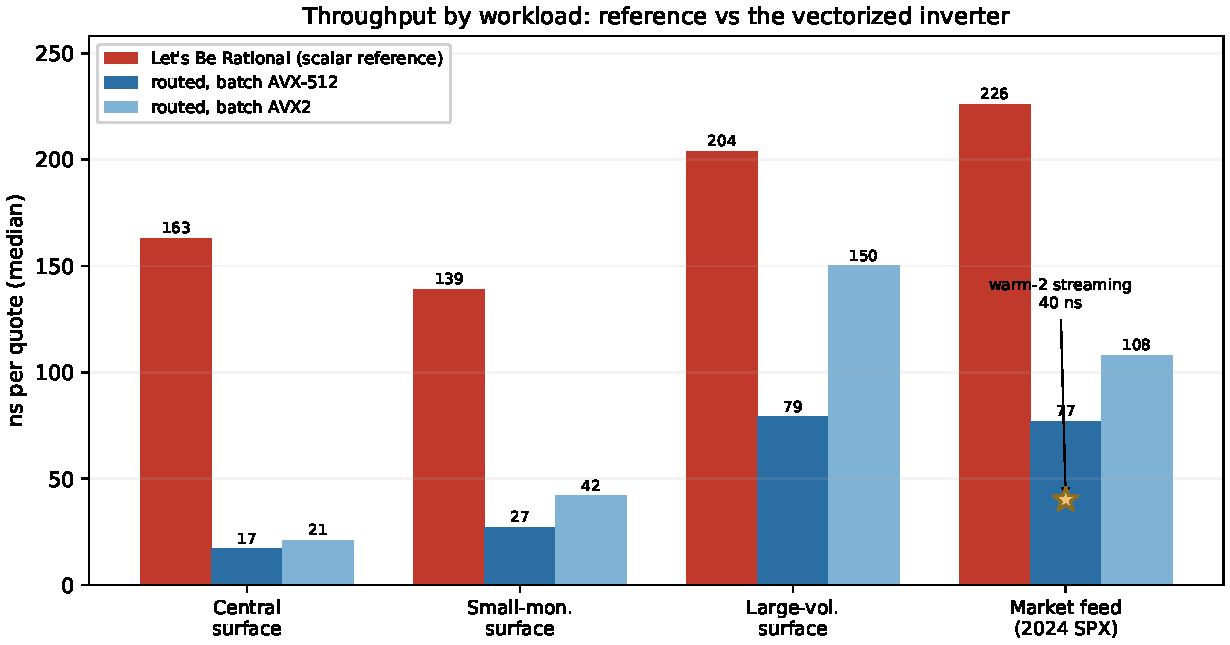
\includegraphics[width=\textwidth]{fig_throughput}
\caption{Median nanoseconds per quote by workload (the data of Table~\ref{tab:timing}), for the scalar reference solver and the routed inverter's two vectorized batch paths (AVX-512 and AVX2). The batch paths are several times faster than the reference on the chart-pure fixed-moneyness batches and on the market-realistic feed. The star marks the warm streaming steady state on the market feed ($40$~ns, AVX-512. Few-ULP warm accuracy contract).}
\label{fig:throughput}
\end{figure}

One throughput property is invisible in medians but operationally significant. The cost per quote is \emph{deterministic}. Every chart executes a fixed operation count (a fixed-degree polynomial sweep, or a fixed number of refinement steps, six Newton in the wing, three Householder at the large-volatility endpoint), so the routed inverter has no iteration-count distribution and no data-dependent tail latency. The slowest quote of a batch costs the same as the median quote of its chart. The reference solver is also fixed-count (a seed and two Householder corrections), so its cost distribution is likewise narrow. The distinction here is not the absence of a tolerance loop but that the fixed count is executed by \emph{branchless} kernels, which is what lets eight quotes advance in lockstep. Solvers that do iterate to a tolerance carry a tail, however short, and hedging pipelines that wait on the last quote of a batch inherit it.

\paragraph{Streaming re-inversion.}
A live system rarely inverts cold twice. The persistent node set of Section~\ref{sec:simd} means every snapshot after the first starts from the previous one. On the market feed, seeding each node with its previous variance after a half-percent move, the guarded two-step warm batch completes in $0.52$ times the cold speculative driver's time on the same feed and host---$40$~ns per quote against the cold driver's $77$ and the reference's $226$. That $5.7\times$ margin is a deployment-mode number, not a method-to-method one---the warm driver is handed each node's previous root, which the cold reference is not, and delivers the warm few-ULP contract---but it is the number a persistent-book system experiences. Having no routing and no deferred drain, its cost is flat in batch size (Figure~\ref{fig:latency}), whereas the cold driver's sort-and-drain overhead only amortizes over batches of a few thousand. The counterpart concerns the single isolated quote. Inverted scalar and cold, one quote at a time, the reference solver remains faster than our scalar entry, whose per-quote context and routing were designed to amortize across a batch. The streaming answer to a single ticked node is therefore the guarded warm refinement of its previous value, not a cold one-off. A caller who genuinely needs isolated cold scalar inversions at minimum latency is the one workload for which the reference remains the better tool.

\begin{table}[t]
\centering
\small
\begin{tabular}{l r r r r}
\toprule
 & \multicolumn{1}{c}{Let's Be} & \multicolumn{3}{c}{Routed inverter, ns per quote} \\
\cmidrule(lr){3-5}
Workload & \multicolumn{1}{c}{Rational} & scalar & batch AVX-512 & batch AVX2 \\
\midrule
Central batch, $h{=}1$              & $163$ & $70$   & $\mathbf{17}$  & $\mathbf{21}$  \\
Small-moneyness batch, $h{=}0.2$    & $139$ & $182$  & $\mathbf{27}$  & $\mathbf{42}$  \\
Large-volatility batch, $h{=}1$     & $204$ & $666$  & $\mathbf{79}$  & $150$ \\
Market feed (2024 SPX, actual prices)& $226$ & $566$ & $\mathbf{77}$  & $\mathbf{108}$ \\
\bottomrule
\end{tabular}
\caption{Median nanoseconds per quote (five repetitions, quiet Intel Core i5-1145G7, Linux, GCC~11.4, \texttt{-O3 -ffp-contract=off -fno-fast-math}), on chart-pure fixed-moneyness batches of $4096$ quotes (fixed $h$, varying price, so kernel benchmarks rather than expiry slices), and on the market-realistic feed of $30{,}000$ actual projected prices resampled from the tradeable 2024 S\&P~500 population (route mix $90/5/5/0$ percent across left/wing/central/right. Mixed $h$, the realistic book workload). The reference column is the author's official public scalar implementation. The market row is timed all-inside (each method pays its own per-quote input transform inside the loop). The fixed-moneyness rows hoist the shared per-$h$ constants. The batch output is bit-identical to the scalar entry on every driver and instruction set (zero mismatches, verified on both the $120{,}000$-point coverage grid and the market feed). Bold marks where the batch beats the reference. Inter-repetition spread was under one percent on every cell.}
\label{tab:timing}
\end{table}

\paragraph{Relation to other methods.}
The natural axes of comparison are accuracy class, domain of validity, and unit of work. The explicit formulas of \citet{li2008approximate}, \citet{stefanica2017explicit} and \citet{xiacui2018exact} are the fastest possible single evaluations and vectorize trivially, but they are approximations valid on bounded regions with accuracy far from the last bit. In the present architecture their natural role is as seeds, and the rational quantile seed of Section~\ref{sec:right} plays exactly that part. \citet{matic2019pde} precompute a polynomial table over moneyness and price, as we do, but target an accuracy of $10^{-7}$. Their open-source C\raise.08ex\hbox{\tt ++}/OpenCL implementation ships a roughly $46$\,MB coefficient file against the present table's $200$\,KB. The gap in accuracy and size has one source. Removing the singular endpoint regimes from the two-dimensional fit lets the central table follow the branch-point principle of Section~\ref{sec:table} instead of refining toward the boundaries. No head-to-head timing is offered, the execution models (GPU/OpenCL versus CPU SIMD) sharing no common harness. \citet{glau2019chebyshev} build a Chebyshev interpolation of the implied-volatility surface as a single global object. Partitioning the domain at the inverse map's branch points is what lets a low, fixed degree hold the last bit out to the boundary of feasibility rather than over a bounded box. \citet{jackel2015rational} remains the accuracy standard, and Table~\ref{tab:accuracy} shows the present method matches it everywhere both are at machine precision, while extending that precision into the two extreme regimes and changing the unit of work from a branchy scalar iteration to a vectorizable fixed-cost evaluation.

\paragraph{Limitations.}
Six boundaries of the claims deserve collection in one place. First, every throughput comparison is against the reference's official public scalar implementation. The correct reading of Table~\ref{tab:timing} is ``faster than what a practitioner can obtain today,'' not ``faster than any conceivable vectorized iteration.'' Second, the route mix ($90\%$ small-moneyness) is one year of one underlying under one tradeability screen. FX, single-name, commodity, or short-dated crypto books, and intraday quote streams, may distribute differently. Third, the batch speedups of Table~\ref{tab:timing} are largest on AVX-512. The AVX2 four-wide twins recover roughly half on the fixed-moneyness batches, though the market-feed advantage ($2.1\times$) survives because every chart including the wing has an AVX2 twin, and hardware without SIMD falls back to the scalar path (still correct, still gated, still bit-identical, not accelerated). Fourth, the machine-precision domain has an explicit edge. The wing tables cover $\beta=h^2/16\le16.4$, i.e.\ $h\le16.2$ (strikes beyond $10^{7}$ times the forward), the rescue branch of Section~\ref{sec:wing} covers the band beyond it (validated for $W\lesssim40$), and the still-deeper corner returns a flagged non-result. For $v>8$ the returned volatility carries the input-representability floor of Section~\ref{sec:setup}, which no double-precision interface can circumvent. Fifth, absolute timings are hardware-specific and a deployment decision should rest on a re-measurement on the target host. The accuracy and bit-identity results, which do not depend on timing conditions, are the load-bearing claims. Sixth, the exhaustive grid validation domain is $\sigma\sqrt T\le8$, $h\le16.5$. The wing evaluator is itself validated on prices to $10^{-320}$, but the grid evidence of Figure~\ref{fig:heat} stops at the stated box.

\paragraph{Reproducibility.}
The oracle scripts, the accuracy and bit-identity harnesses, the benchmark driver, the market-feed sample and the frozen table are provided as supplementary material, with build lines for all three instruction-set targets. Appendix~\ref{app:artifacts} lists the artifacts. A golden-vector verifier (oracle-checked $(h,c)\to w$ triples spanning every chart and seam) lets an adopter confirm, in one command after building, that their compiler and hardware reproduce both the accuracy gate and the bit-identity invariant. Every number in this section is regenerated by the harnesses from the shipped sources.

\section{Conclusion}
\label{sec:conclusion}

Recovering implied volatility to machine precision is a solved problem for a single scalar quote. What has been missing is a method that reaches that precision through an evaluation that also vectorizes over the whole feasible domain. The routed table inverter presented here supplies one. A branch-point-sized central Chebyshev table and three matched endpoint charts, unified by a single two-parameter special-function family, resolve every feasible quote by routed evaluation with fixed-count local refinement, and branchless kernels shared between the scalar and SIMD paths make five distinct builds (two compilers, three instruction sets) return bitwise-identical doubles on every validation quote. The worst relative error observed against a 40-digit oracle is $8.3\times10^{-16}$, held into the near-intrinsic and deep-wing regimes where the reference solver degrades, and every representable input receives a full-accuracy result or a flagged non-result. On a market-realistic S\&P~500 book the batch drivers run at $2.1$--$2.9$ times the scalar reference, and the guarded warm refinement of a persistent book roughly doubles that again under its few-ULP contract. Since both solvers are at machine precision on tradeable quotes, the practical case is throughput and determinism, with the accuracy margin as insurance at the extremes. The natural extensions are a Bachelier (normal-volatility) analogue, for which the same routed-chart architecture applies with the normal density in place of the log-normal, and a data-parallel GPU port, for which the fixed-cost, branch-light kernel structure is well suited.

\newpage
\bibliographystyle{apalike}
\bibliography{refs}

\newpage
\appendix
\section*{Appendix}
\addcontentsline{toc}{section}{Appendix}

\section{The hot path}
\label{app:hotpath}

The complete scalar evaluation, which the batch drivers reproduce bucket-wise, is the following. All constants are frozen doubles. $\mathrm{bits}(\cdot)$ denotes IEEE-754 bit extraction, and $\log_2^{*}$ is the shared logarithm kernel of Section~\ref{sec:simd}.

\medskip\noindent\textbf{Routing} (given $h\ge0$ and $c\in(0,1)$):
\begin{enumerate}[leftmargin=2em,itemsep=1pt]
\item if $h=0$: solve the exact ATM relation $c=\erf(\sigma/2\sqrt2)$ (quantile seed, two guarded corrections). Return. \item if $c<c_{\mathrm{wing}}(h)$ (one Chebyshev in $h$): \textsc{Wing}. \item if $h<0.3$: \textsc{Left} if $c\le c_{\mathrm{tl}}(h)$ (a frozen degree-$8$ Chebyshev fit of $C(h,1.70)$, so the test is a polynomial, not a price evaluation), else \textsc{Right}. \item if $h\le H_{\mathrm{box}}$ and $c\le c_2(h)$: \textsc{Central}. Else \textsc{Right}.
\end{enumerate}

\medskip\noindent\rtag{Central} (table): band from $\mathrm{bits}(h)$. Octave and sub-cell from $\mathrm{bits}(c)$; $x_\lambda=\alpha_{\mathrm{cell}}\log_2^{*}(m)+\beta_{\mathrm{cell}}$ with $m$ the mantissa of $c$; $W$ by the bivariate Clenshaw sweep \eqref{eq:cheb2}. Return $w=h^2/(2W)$.

\medskip\noindent\rtag{Left}: $\rho=c/\expmone(h)$; $A=B^{-1}(\rho)$ (three-regime Chebyshev); $s=h/A$; $v=v_0(\kappa s)+h^2V_2(s)+h^4V_4(s)+h^6R(s,h)$. Return $w=v^2$.

\medskip\noindent\rtag{Right}: $\bar g=\tfrac12(1-c)e^{-h/2}$; $x_0=-\Phi^{-1}_{\mathrm{seed}}(\bar g)$ (rational seed); Mills ratio $m_0=\sqrt{\pi/2}\;\erfcx(x_0/\sqrt2)$. Ladder corrections $x=x_0+h^2x_2+h^4x_4$ with $x_2,x_4$ polynomial in $1/x_0,m_0$. Then exactly three Householder-3 steps on \eqref{eq:rightchart}, with $f/g'$ from \eqref{eq:gprime} and the closed-form ratios $g''/g'=-x+h^2/(4x^3)$, $g'''/g'=(g''/g')^2-1-3h^2/(4x^4)$, prices evaluated in whichever of $c$, $1-c$ is small. Return $w=(2x)^2$.

\medskip\noindent\rtag{Wing}: if $h^2/16>16.4$: rescue branch ($\PhiN$-inversion seed, three fixed-point corrections, three Householder steps. Quiet NaN beyond its validated band). Otherwise $\widetilde L$ from $\log c$ (subnormal-safe $\log_2^{*}$) and $h$. Regime (piece A / piece B / series) once from $\widetilde L$. Exactly six Newton steps on $W=\widetilde L-\tfrac32\log W+\log H(W)$ with $\log H$ and its analytic derivative from the fitted $S(u,\beta)$ (or the series). Return $w=h^2/(2W)$.

\medskip\noindent\textbf{Batch drivers}: a strided moneyness sample selects one of two paths. \emph{Speculative} (small-moneyness-heavy feeds, the live case): stream eight/four-wide. Classify each lane by the frozen seam polynomials. Evaluate the small-moneyness kernel on every lane. Masked-store the small-moneyness lanes in input order. Compress the rest into a deferred buffer. \emph{Sort-then-batch} (the deferred buffer, and minority-dominated feeds): classify, counting-sort by cell, chart and wing regime, and evaluate each bucket eight/four-wide. Both are bit-identical to the scalar entry, so the dispatch changes only speed. Remainders, the rescue branch and the ATM line go through the scalar entry unchanged.

\section{Table generation and validation}
\label{app:generation}

The offline pipeline that produces the frozen constants is as important to the accuracy claim as the runtime, so we record it.

\begin{enumerate}[leftmargin=2em,itemsep=1pt]
\item \emph{Truth generation.} For each cell, Chebyshev nodes in $(x_h,x_\lambda)$ are mapped to exact double-precision prices, and each price is inverted by an arbitrary-precision solver (no fewer than 25 significant digits, price residual driven below $10^{-18}$). The transformed truth $W=h^2/(2w)$ is recorded. \item \emph{Fitting.} Tensor Chebyshev coefficients are computed per cell. Degrees are the smallest passing the gate below, capped at $(13,16)$. \item \emph{Gating.} An independent 40-digit oracle, sharing no code with the generator, re-inverts a dense sample of each cell including its boundaries and the sub-cell seams. The cell is accepted only if the relative $\sigma$ error is below $10^{-15}$ at every sample. Failing cells are refit at higher degree or split. The same gate validates every auxiliary kernel ($\log_2^{*}$, $v_0$, $B^{-1}$, $V_2$, $V_4$, $\erfcx$, the exponential, the residual $R$), with the additional downstream-degree criterion of Section~\ref{sec:simd}. \item \emph{Freezing.} Accepted coefficients are emitted as exact hexadecimal doubles into a header. The runtime contains no fitted constant that did not pass the gate.
\end{enumerate}

Certified enclosures for the endpoint functions are available independently of the gate through the Stieltjes representation of Section~\ref{sec:unify}, whose continued-fraction convergents bound $B$, $B_n$ and $B^{-1}$ from alternating sides.

For the benefit of implementers we also record the design alternatives that the gate \emph{rejected}, since each looks attractive on paper. A transcendental-free table in the raw mantissa coordinate (routing and abscissa both from bit fields, no logarithm at all) fails on degree. The $h$-independent branch-point distances of Section~\ref{sec:table} pin the Bernstein parameter and roughly double the degree per cell, blowing the byte budget. A conformal coordinate adapted to the annulus fails the same way, more severely. Evaluating the cells in the monomial basis with Estrin's scheme, instead of Chebyshev with Clenshaw's, fails the precision gate outright at the required degrees. An equal-accuracy minimax replacement for the logarithm kernel fails through the downstream-degree effect described in Section~\ref{sec:simd}. Fitting the wing's $\log H$ directly, or its unweighted peeled residual, demands degrees past thirty-six where the $\sigma$-weighted form needs twenty-six, and a $(1/W,\beta/W)$ chart for the same fit, natural-looking because $\beta/W=v^2/8$ is bounded, brings no degree reduction because the hard structure at the small-$W$ edge is genuinely asymptotic rather than an artifact of coordinates. Finally, one accepted choice had to be revised by a denser gate. Five wing Newton steps passed a sparse step-count de-risk yet left six points of the dense regular grid above $10^{-15}$ (worst $1.2\times10^{-14}$), all at the high-$\beta$, low-$W$ corner where convergence is slowest. The fixed count is six, and the incident is a reminder that step-count de-risking must sample the corner of slowest convergence, not the typical point. Each rejection was measured, not argued.

\section{Artifacts}
\label{app:artifacts}

The supplementary material contains: the header-only C\raise.08ex\hbox{\tt ++}17 implementation (runtime, frozen tables, wing evaluator, checked API). The oracle generators (\texttt{mpmath}, 40 digits) for the regular, stressed and edge sets. The golden-vector verifier and its oracle file (the one-command build check of Section~\ref{sec:results}). The accuracy harness producing Table~\ref{tab:accuracy}, Table~\ref{tab:edge} and Figure~\ref{fig:heat}. The bit-identity and poison-test harnesses. The market-feed sample ($30{,}000$ pairs $(h,c)$ resampled from the tradeable 2024 population, where $c$ is the \emph{actual} parity-projected quote price normalized per Section~\ref{sec:setup} (tick rounding and spread noise included, not prices regenerated from fitted volatilities), exactly the bytes the timed market rows consume), and the throughput benchmark, including the build lines for the AVX-512, AVX2 and scalar targets used in Section~\ref{sec:results}. The feed derives from a licensed OptionMetrics file, so the supplement carries only these transformed pairs together with the filter and projection recipe needed to regenerate them from a licensed copy. For independent audit, the closed forms of $V_2$ and $V_4$, the ladder coefficients $B_n$, the frozen seam and wing fits, and the exact residual equations driving the Householder and Newton refiners appear in the shipped headers in the notation of the text. The reference implementation of \citet{jackel2015rational} (revision~$1520$, obtained from \url{http://www.jaeckel.org/}) is the version current when the benchmarks were run and is linked unmodified. One portability note deserves record. A code-generation defect in one Windows GCC toolchain (misaligned vector spills in a heavily spilled function, affecting AVX-512 and AVX2 builds alike and unrelated to this code's logic) can crash the mixed-grid driver on that platform. The artifacts document the affected configuration, and all results here are from Linux, which is unaffected.

\end{document}
